\documentclass[a4paper]{article}

%% Must have
\usepackage[T1]{fontenc}
\usepackage[utf8]{inputenc}
\usepackage{float}
\usepackage{graphicx}

%% Style
\usepackage[english]{babel}
\usepackage{multicol}
\usepackage{cite}
\usepackage{hyperref}
\usepackage{url}
\usepackage{booktabs} % http://ctan.cs.uu.nl/macros/latex/contrib/booktabs/booktabs.pdf
\usepackage{fancyhdr}
\usepackage{cite}
\usepackage[nottoc,numbib]{tocbibind} % number references
\usepackage[a4paper]{geometry} % a4 margins
\clubpenalty = 10000
\widowpenalty = 10000 % Avoid dangling sentences
\usepackage{subfig}   %\subfloat[][]{\includegraphics{...}\label{fig:1}}
                      %\subfloat[][]{\includegraphics{...}\label{fig:2}} \caption{\subref{fig:1} blabla. \subref{fig:2} blabla.}
                      % \caption{\subref{fig:1} blabla. \subref{fig:2} blabla.}
\usepackage[usenames,dvipsnames,svgnames,table]{xcolor}

%% Math
\usepackage{amsmath}
\usepackage{amssymb}
\usepackage{bm}


%% Typography
\usepackage{kpfonts}
\usepackage{beramono}
\usepackage{microtype} % load after font

%% Listings
\usepackage{listings}
\lstset{%
    language         = Python,
    basicstyle       = \ttfamily\footnotesize,
    keywordstyle     = \bfseries\color{blue},
    stringstyle      = \color{magenta},
    commentstyle     = \color{ForestGreen},
    showstringspaces = false,
    aboveskip={0.9\baselineskip},
    belowskip={0.9\baselineskip},
    columns=fixed,
    extendedchars=true,
    frame=lines,
}

\pagestyle{fancy}
\fancyhf{}
\rhead{Joris van Vugt}
\lhead{Statistical Machine Learning (NWI054E)} % Project etc.
\rfoot{\thepage}

\author{Joris van Vugt, s4279859}
\title{Statistical Machine Learning: Assignment 4} % Title
\date{\today}

\begin{document}
\maketitle
\section*{Exercise 1 -- Gaussian processes for regression} %%%%%%%%%%%%%%
\begin{enumerate}
\item The following code implements a vectorized implementation of the kernel. The entire dataset can be processed with a single call.

\begin{lstlisting}
def kernel(a, b, theta):
    sqdist = np.sum(a**2, axis=1) + np.sum(b**2, axis=1) - 2*np.dot(a, b.T)
    return theta[0]*np.exp(-theta[1]/2 * sqdist) + theta[2] + theta[3]*a.dot(b.T)
\end{lstlisting}

\item The following code creates a column vector $\bm{X}$ of $N=101$ equally spaced points between $-1$ and $1$ (inclusive). It then computes the Gram matrix $\bm{K}(\bm{X}, \bm{X})$ with parameter vector $\bm{\theta}=[1, 1, 1, 1]$.
\begin{lstlisting}
N = 101
theta = np.ones(4)
X = np.linspace(-1, 1, N).reshape(N, 1)
K = kernel(X, X, theta)
\end{lstlisting}
\item $\bm{K}$ is an $N \times N$ matrix with $\bm{K}_{ij} = k(\bm{X}_i, \bm{X}_j)$. We can show that $\bm{K}$ is positive semidefinite by showing that all eigenvalues are larger or equal to zero. Because of numerical issues, we have a small tolerance. It turns out that the smallest eigenvalue is in fact $-1.5\times10^{-14}$.
\begin{lstlisting}
def is_psd(A, tol=1e-8):
    eigen, _ = np.linalg.eigh(A)
    return np.all(E > -tol)

is_psd(K) # -> True
\end{lstlisting}
Additionally, $k$ can be shown to be a valid kernel using equations 6.13-6.22 from Bishop.

\item We can use the Gram matrix $\bm{K}(\bm{X}, \bm{X})$ to sample functions from the Gaussian process prior $\bm{y}(\bm{X}) \sim \mathcal{N}(\bm{0}, \bm{K}(\bm{X}, \bm{X}))$. See Figure \ref{fig:sampled_f}.

\begin{lstlisting}
mu = np.zeros(N)
for _ in range(5):
    plt.plot(np.random.multivariate_normal(mu, K))
plt.show()
\end{lstlisting}

\begin{figure}
\centering
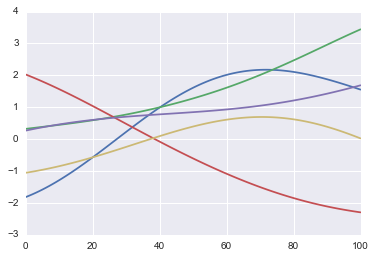
\includegraphics[width=.5\linewidth]{figures/sampled_f.png}
\caption{5 functions sampled from the Gaussian process prior.}
\label{fig:sampled_f}
\end{figure}

\item Figure \ref{fig:sample_thetas} shows functions sampled using different settings of $\theta$.

\textbf{Bonus}: $\theta_0$ influences the overall scale of the function. The higher $\theta_0$, the higher the absolute range of the function. For example, the functions in the second plot have a much higher range than in most other plots.\\
A small $\theta_1$ makes the function very smooth (e.g., plot 4), while a high $\theta_1$ makes the function more jagged (e.g., plot 3). \\
$\theta_2$ once again controls the range of the function (e.g., plot 5). \\
$\theta_3$ influences both the smoothness and the range of the function, since it controls the weight of the dot-product of the inputs.

\begin{figure}
\centering
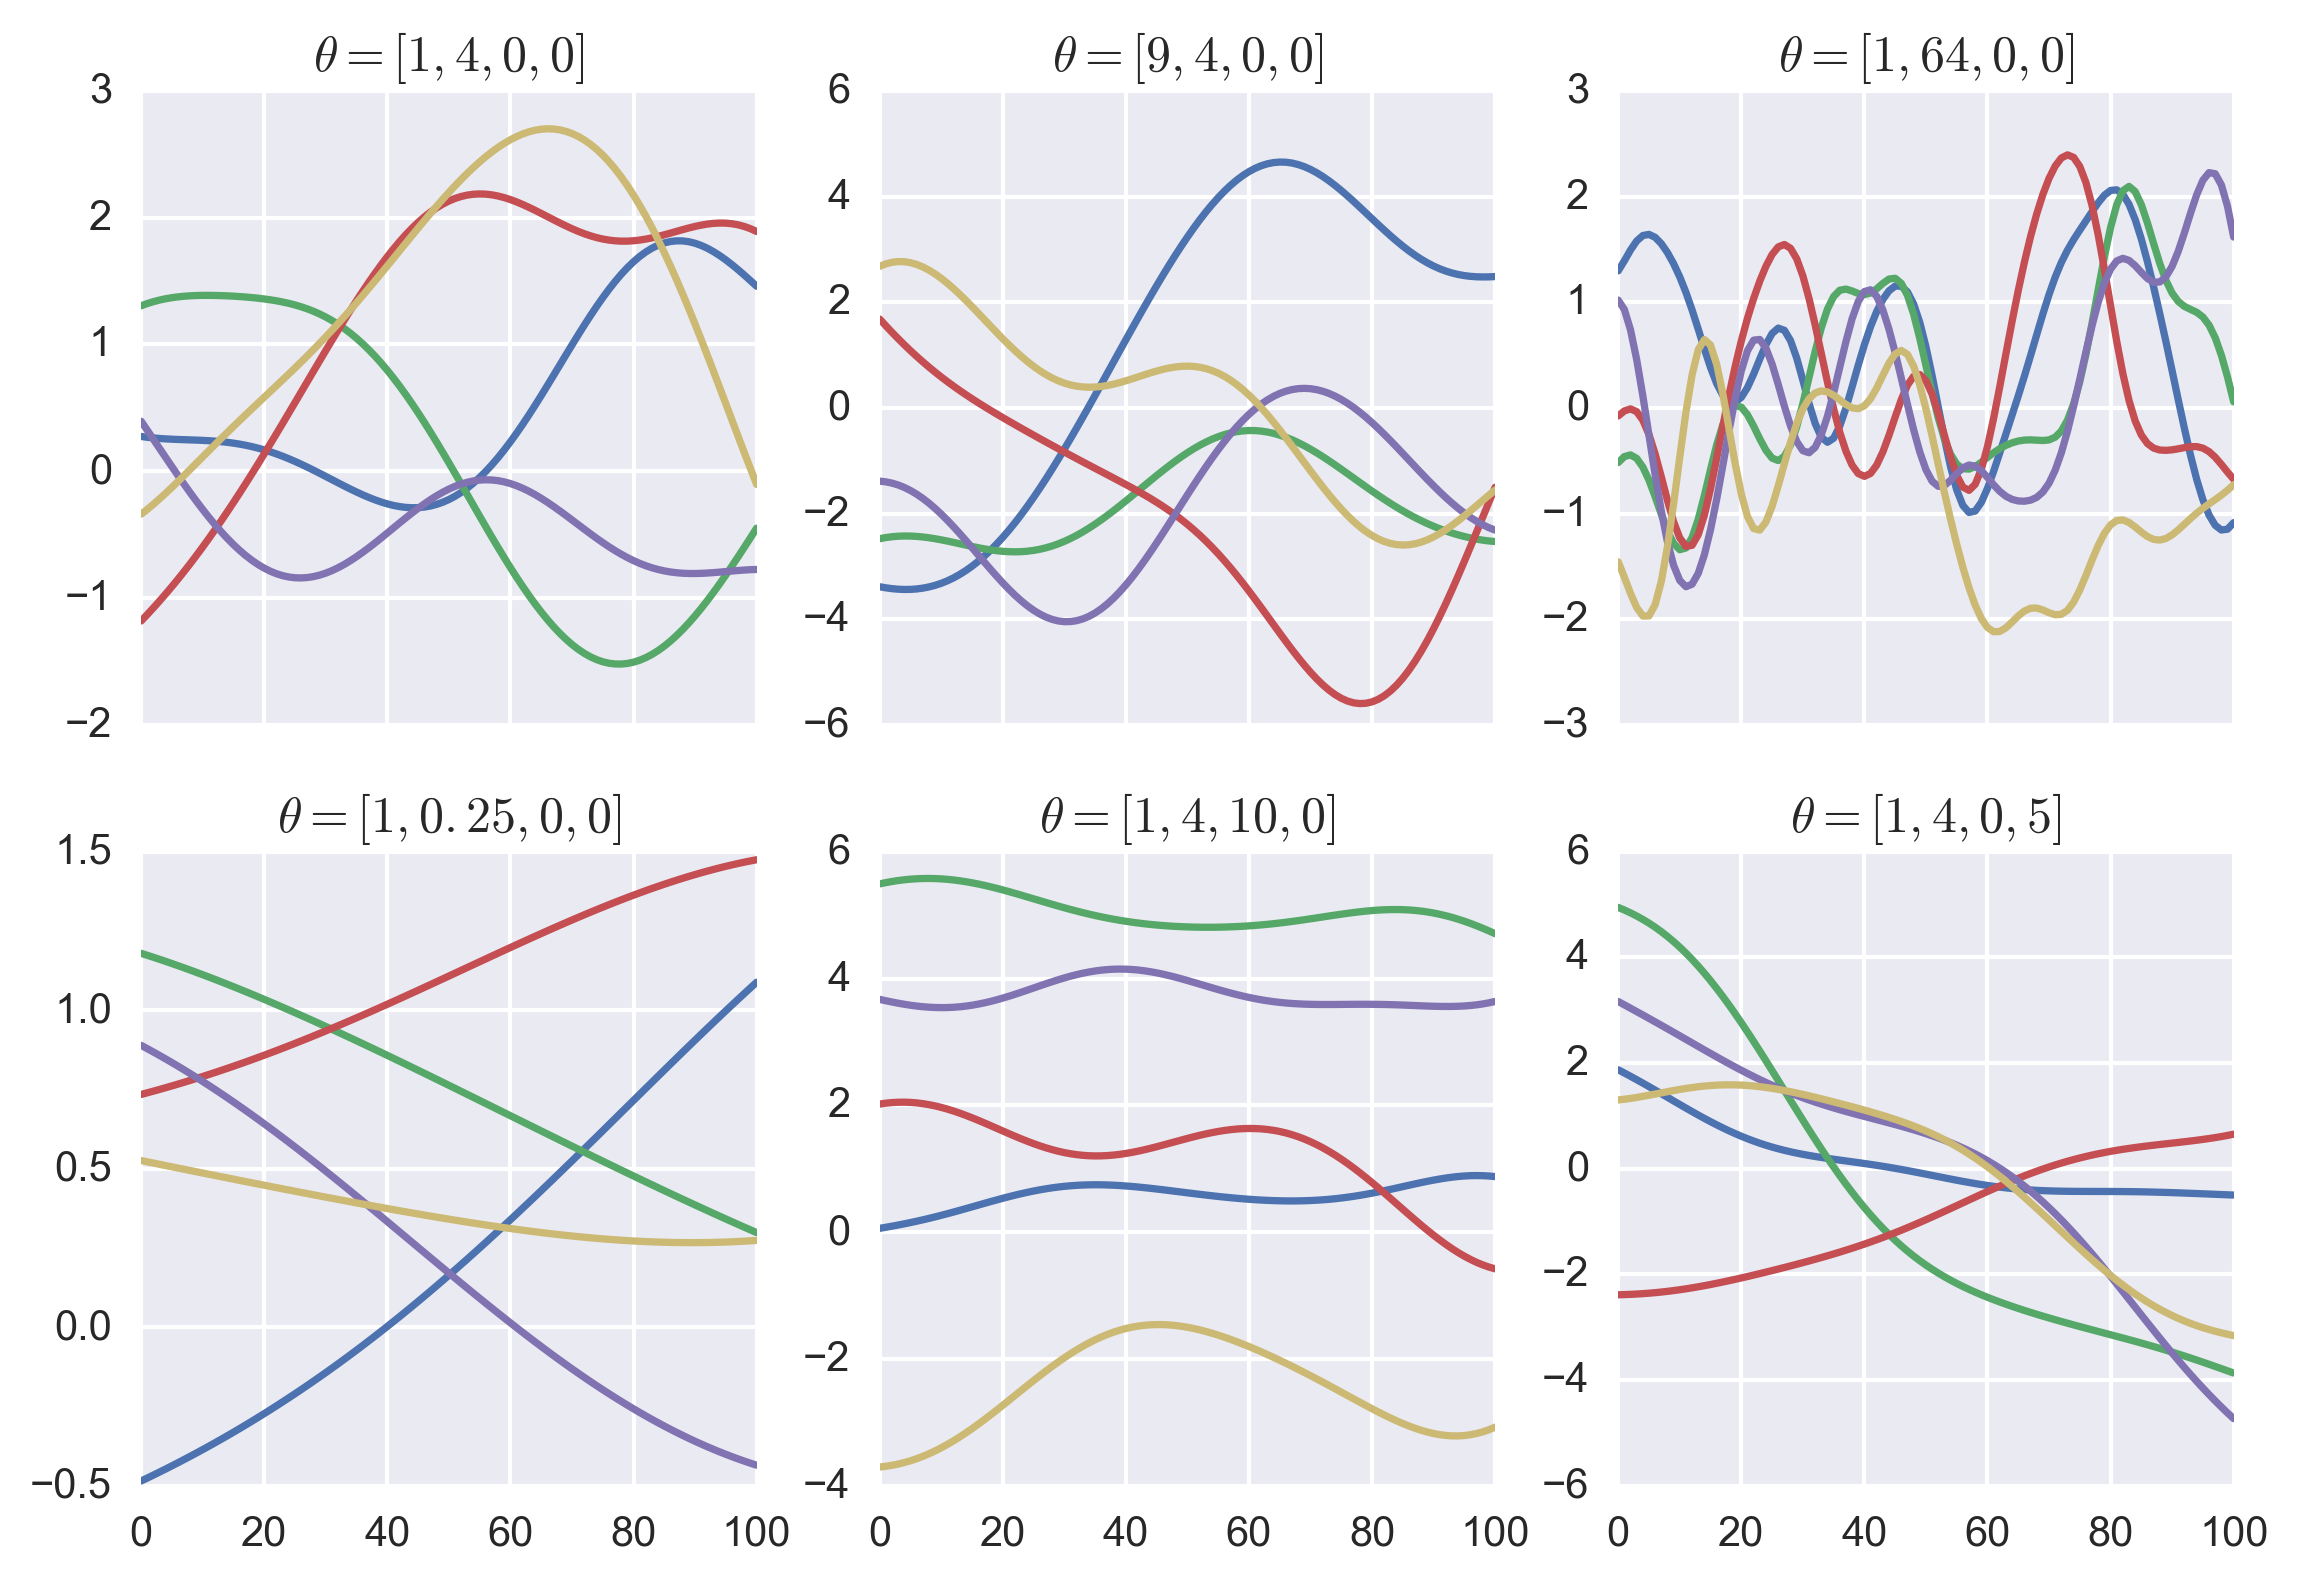
\includegraphics[width=.8\linewidth]{figures/sample_thetas.png}
\caption{5 functions sampled from the Gaussian process prior using different kernel parameters.}
\label{fig:sample_thetas}
\end{figure}


\item 
We first compute the Gram matrix
\begin{equation*}
\bm{K} = 
\begin{pmatrix}
2.25 & 1.68 & 1.58 & 1.97 \\
1.68 & 2.04 & 2.06 & 1.94 \\
1.58 & 2.06 & 2.09 & 1.89 \\
1.97 & 1.94 & 1.89 & 2.01
\end{pmatrix}.
\end{equation*}
Next, we can compute the covariance matrix $\bm{C}$ corresponding to the marginal distribution of the training target values $p(\bm{t}) = \mathcal{N}(\bm{t}|\bm{0}, \bm{C})$

\begin{align}
C(\bm{x}_n, \bm{x}_m) &= k(\bm{x}_n, \bm{x}_m) + \beta^{-1}\delta_{nm} \\
\bm{C} &= \bm{K} + \beta^{-1}\bm{I} \\
\bm{C} &= 
\begin{pmatrix}
3.25 & 1.68 & 1.58 & 1.97 \\
1.68 & 3.04 & 2.06 & 1.94 \\
1.58 & 2.06 & 3.09 & 1.89 \\
1.97 & 1.94 & 1.89 & 3.01 \nonumber
\end{pmatrix}.
\end{align}


\item To compute the mean and standard deviation of $p(t|\bm{t})$ for $x=0$, we need equations 6.65, 6.66 and 6.67 from Bishop.
\begin{align}
\bm{C}_{N+1} &= \begin{pmatrix}\bm{C}_N & \bm{k} \\ \bm{k}^T & c\end{pmatrix} \\
m(\bm{x}_{N+1}) &= \bm{k}^T\bm{C}_N^{-1}\bm{t}=-0.25 \\
\sigma^2(\bm{x}_{N+1}) &= c - \bm{k}^T\bm{C}_N^{-1}\bm{k}=0.23
\end{align}


\item The mean of the conditional distribution $p(t|\bm{t})$ does not go to zero in the limit $x \rightarrow \pm\infty$. This is because $k$ is a function of $x$ and has a constant term. If we set $\theta_2 = \theta_3 = 0$, the mean does in fact go to zero.

\end{enumerate}


\pagebreak
\section*{Exercise 2 -- Neural network regression} %%%%%%%%%%%%%%%%%%%%%%
\begin{enumerate}
\item The gaussian shown in Figure \ref{fig:mvg} is created with the following code
\begin{lstlisting}
X = np.mgrid[-2:2:.1, -2:2:.1]
y = 3 * multivariate_normal(np.zeros((2,)), 0.4*np.eye(2)).pdf(X.T)

fig = plt.figure(figsize=(10, 10), dpi=300)
ax = fig.gca(projection='3d')
col = ax.plot_surface(X[0], X[1], y, cmap=plt.cm.viridis, rstride=3, cstride=3)
plt.xlabel('$x_1$')
plt.ylabel('$x_2$')
ax.set_zlabel('$p(x_1, x_2)$')
plt.colorbar(col)
plt.savefig('mvg.png', bbox_inches='tight', dpi=300)
plt.show()
\end{lstlisting}
\begin{figure}
\centering
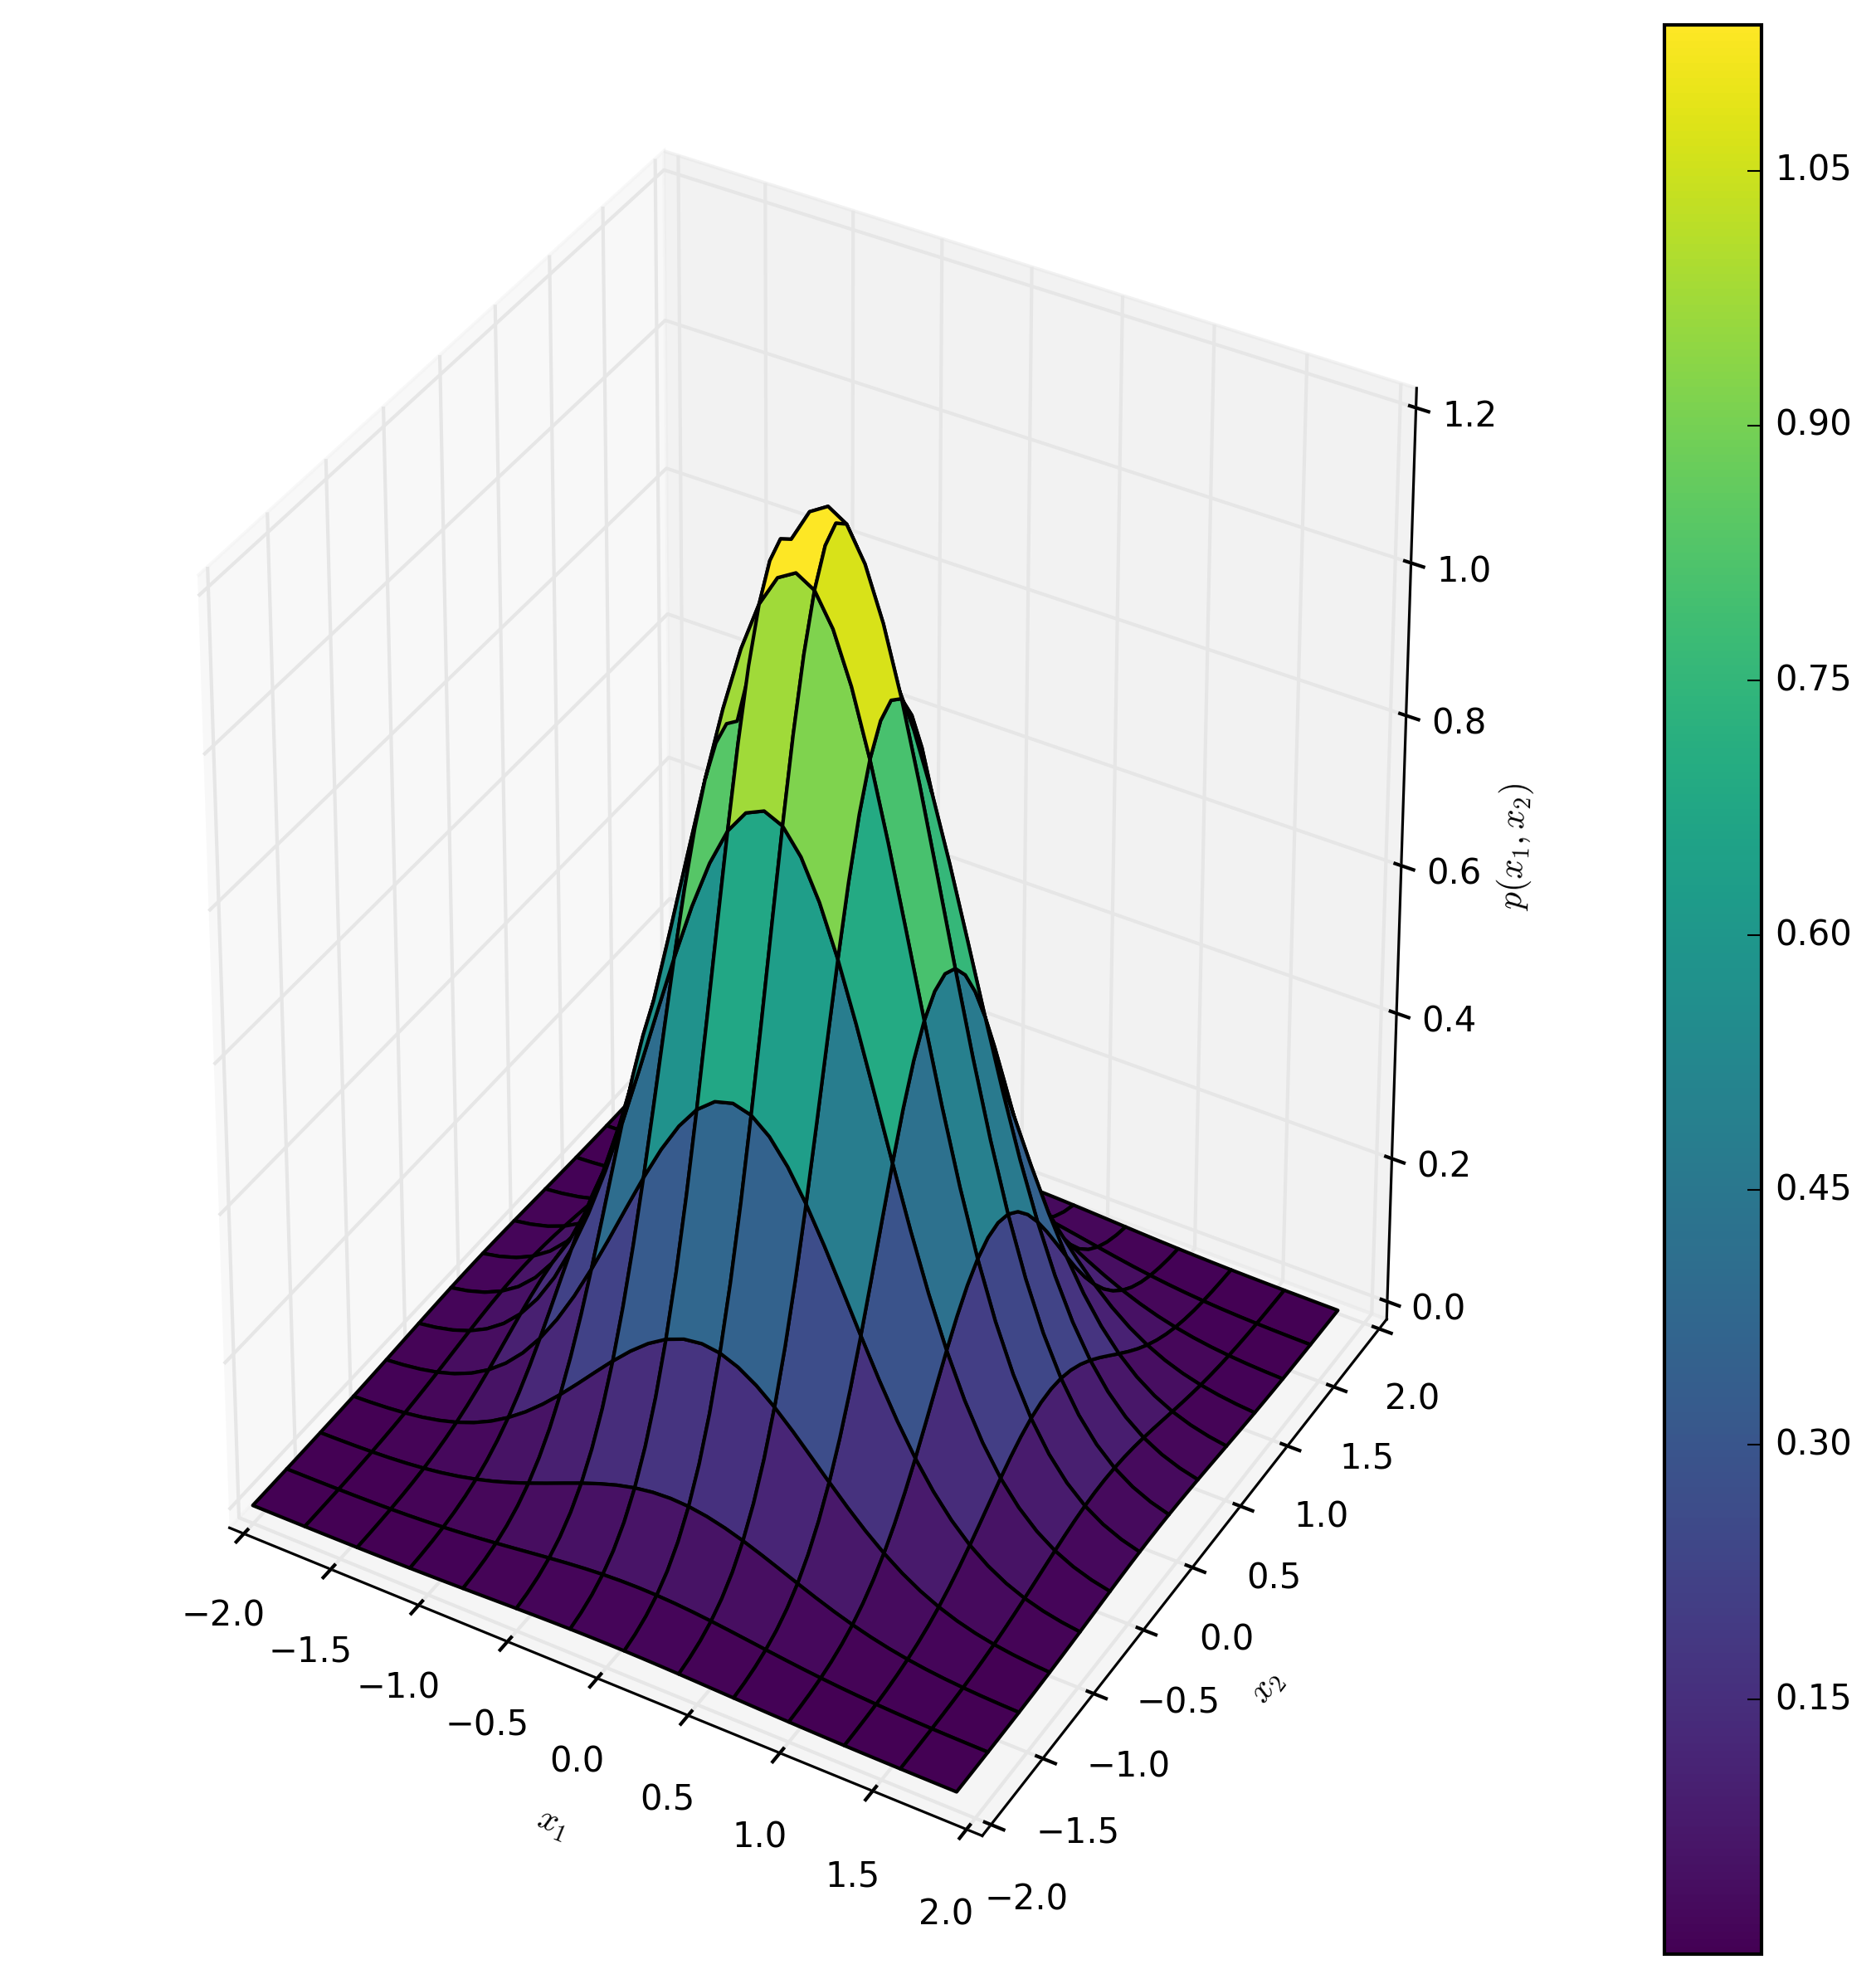
\includegraphics[width=.8\linewidth]{figures/mvg.png}
\caption{An isotropic 2D gaussian given by $y = 3 \cdot \mathcal{N}(\bm{x}|\bm{0}, \frac{2}{5}\bm{I}_2)$}
\label{fig:mvg}
\end{figure}
\item The following class implements the multi-layer perceptron described in the assignment. It is able to process an entire batch of data simultaneously. However, because of the sum-of-squares error function, the error quickly becomes very large, which is impractical for training.
\begin{lstlisting}
class MultiLayerPerceptron():
    def __init__(self, D=2, K=1, M=2, learning_rate=0.1):
        self.learning_rate = learning_rate
        self.D, self.K, self.M = D, K, M
        
        
        model = {}
        model['W1'] = np.random.uniform(low=-0.5, high=0.5, size=(D, M))
        model['b1'] = np.zeros(M)
        model['W2'] = np.random.uniform(low=-0.5, high=0.5, size=(M, K))
        model['b2'] = np.zeros(K)
        self.model = model
        
    def forward(self, X):
        """
        X has shape [N x 2]
        Returns the predictions for X [N, 1] and cached variables
        for backprop
        """
        h_in = np.dot(X, self.model['W1']) + self.model['b1']
        h = np.tanh(h_in)
        y = np.dot(h, self.model['W2']) + self.model['b2']
        return y, {'X': X, 'h': h, 'W2': self.model['W2']}
    
    def backward(self, dout, cache):
        """
        dout is the gradient on the loss function wrt to the predictions
        cache is a dictionary of variables
        """
        grads = {}
        grads['W2'] = np.dot(cache['h'].T, dout)
        grads['b2'] = np.sum(dout, axis=0)
        dh = np.dot(dout, cache['W2'].T)
        dh_in = (1 - cache['h']**2) * dh # backprop through tanh
        grads['W1'] = np.dot(cache['X'].T, dh_in)
        grads['b1'] = np.sum(dh_in, axis=0)
        return grads
    
    def loss(self, preds, y):
        """
        Computes the sum of squares error
        """
        difference = preds - y.reshape(-1, 1)
        error = 0.5 * np.sum(difference**2)
        return error, difference
    
    def train(self, X, y, iterations=500, verbose=True):
        for i in range(iterations):
            preds, cache = self.forward(X)
            cost, dpreds = self.loss(preds, y)
            grads = self.backward(dpreds, cache)
            if verbose:
                print('Iteration %d: loss=%.4f' % (i, cost))
            for param in self.model.keys():
                self.model[param] -= grads[param] * self.learning_rate
\end{lstlisting}
The initial weights yield the ``distribution'' shown in Figure \ref{fig:init_dist}. As to be expected, it doesn't look much like the original distribution yet.

\begin{figure}
\centering
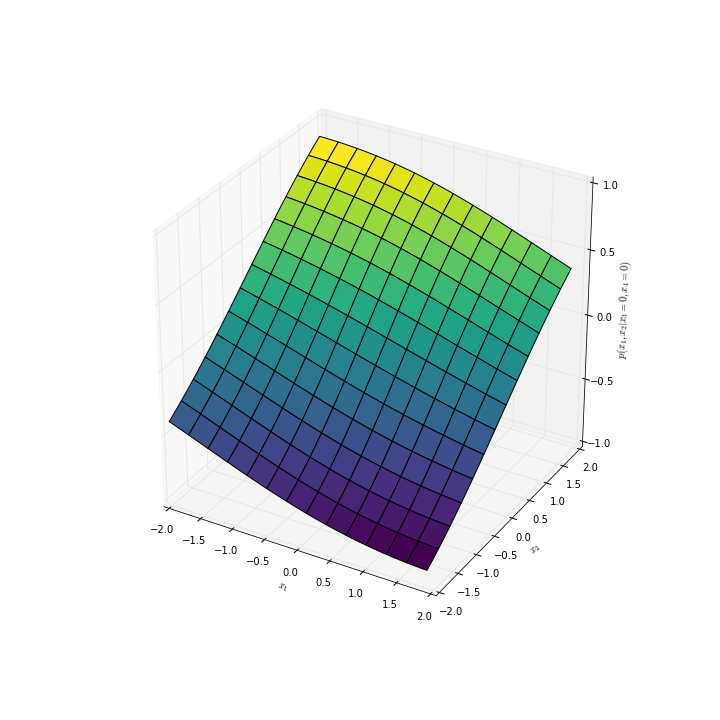
\includegraphics[width=.8\linewidth]{figures/initial_dist.png}
\caption{The output of the MLP after random initialization (i.e., no training).}
\label{fig:init_dist}
\end{figure}

\item After 200 iterations the output indeed starts to resemble a gaussian. However, the loss also shows that the minimal loss was also reached around that point. See Figure \ref{fig:mvg200}.

\begin{figure}
\centering
\subfloat[The output of the network after 200 iterations.]{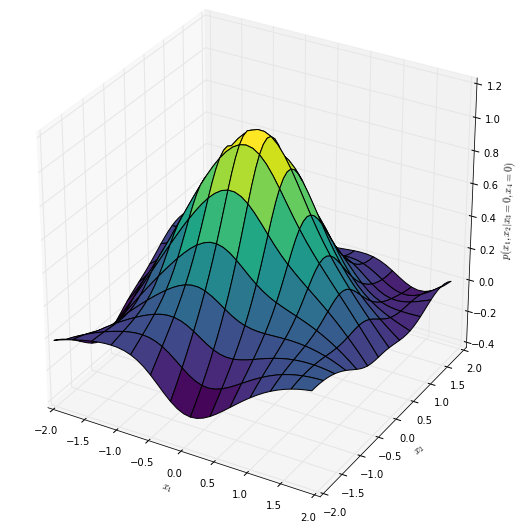
\includegraphics[width=.48\linewidth]{figures/mvg200.png}}
\subfloat[The loss as a function of the number of iterations.]{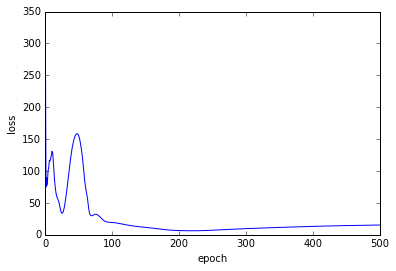
\includegraphics[width=.48\linewidth]{figures/loss.png}}
\caption{The training process of an MLP with $M=8$ and $\eta=0.1$.}
\label{fig:mvg200}
\end{figure}


\item Randomly permuting $\bm{X}$ and $\bm{Y}$ drastically increases both the speed of convergence and the quality of the final model (see Figure \ref{fig:perm}. The final loss is $0.54$. The reason for this is that the model doesn't overfit as much to specific areas of the gaussian. If the data isn't permuted, the network will see a lot of similar samples sequentially. It will then overfit on this particular area and perform worse on other areas of the gaussian.

Increasing the number of hidden units will further increase the loss (e.g., $M=40$ yields a loss of $0.07$). If the network has more hidden units, it will have more expressive power. The number of weights will also increase, so the weights take longer to converge.

Decreasing the learning rate to $0.01$ increases the time it takes to converge. However, there is less noise in the loss over time and the final loss is lower ($1.03$). With a lower learning rate, gradient descent can make more subtle moves in the loss landscape. This leads to better optima.

Different initial weights only slightly effect the final performce of the network.

\begin{figure}
\centering
\subfloat[The final output of the network.]{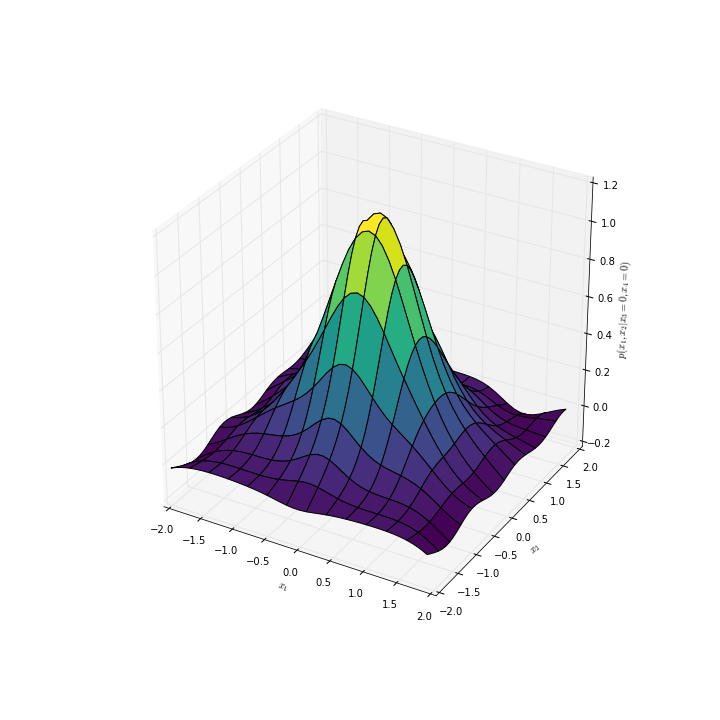
\includegraphics[width=.48\linewidth]{figures/perm.png}}
\subfloat[The loss as a function of the number of iterations.]{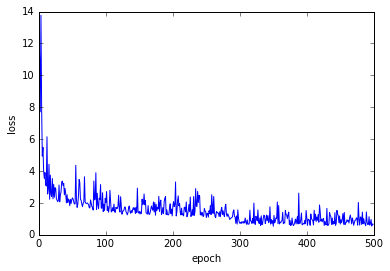
\includegraphics[width=.48\linewidth]{figures/perm_loss.png}}
\caption{The training process of an MLP with $M=8$ and $\eta=0.1$ with the input randomly permuted.}
\label{fig:perm}
\end{figure}

\item In Python, a little bit more work is required to plot the desired density (Figure \ref{fig:mm}).
\begin{lstlisting}
def plot_density(X, Y):
    fig = plt.figure(figsize=(10, 10), dpi=300)
    ax = fig.gca(projection='3d')
    ax.plot_surface(X[:, 0].reshape(41, 41), X[:, 1].reshape(41, 41), Y.reshape(41, 41), 
                    cmap=plt.cm.viridis, rstride=1, cstride=1, linewidth=1)
    plt.xlabel('$x_1$')
    plt.ylabel('$x_2$')
    ax.set_zlabel('$p(x_1, x_2)$')
    ax.view_init(30, 230)
    plt.show()
\end{lstlisting}

\begin{figure}
\centering
\subfloat[The multi-modal probability density to be modelled in the second part of the second exercise.]{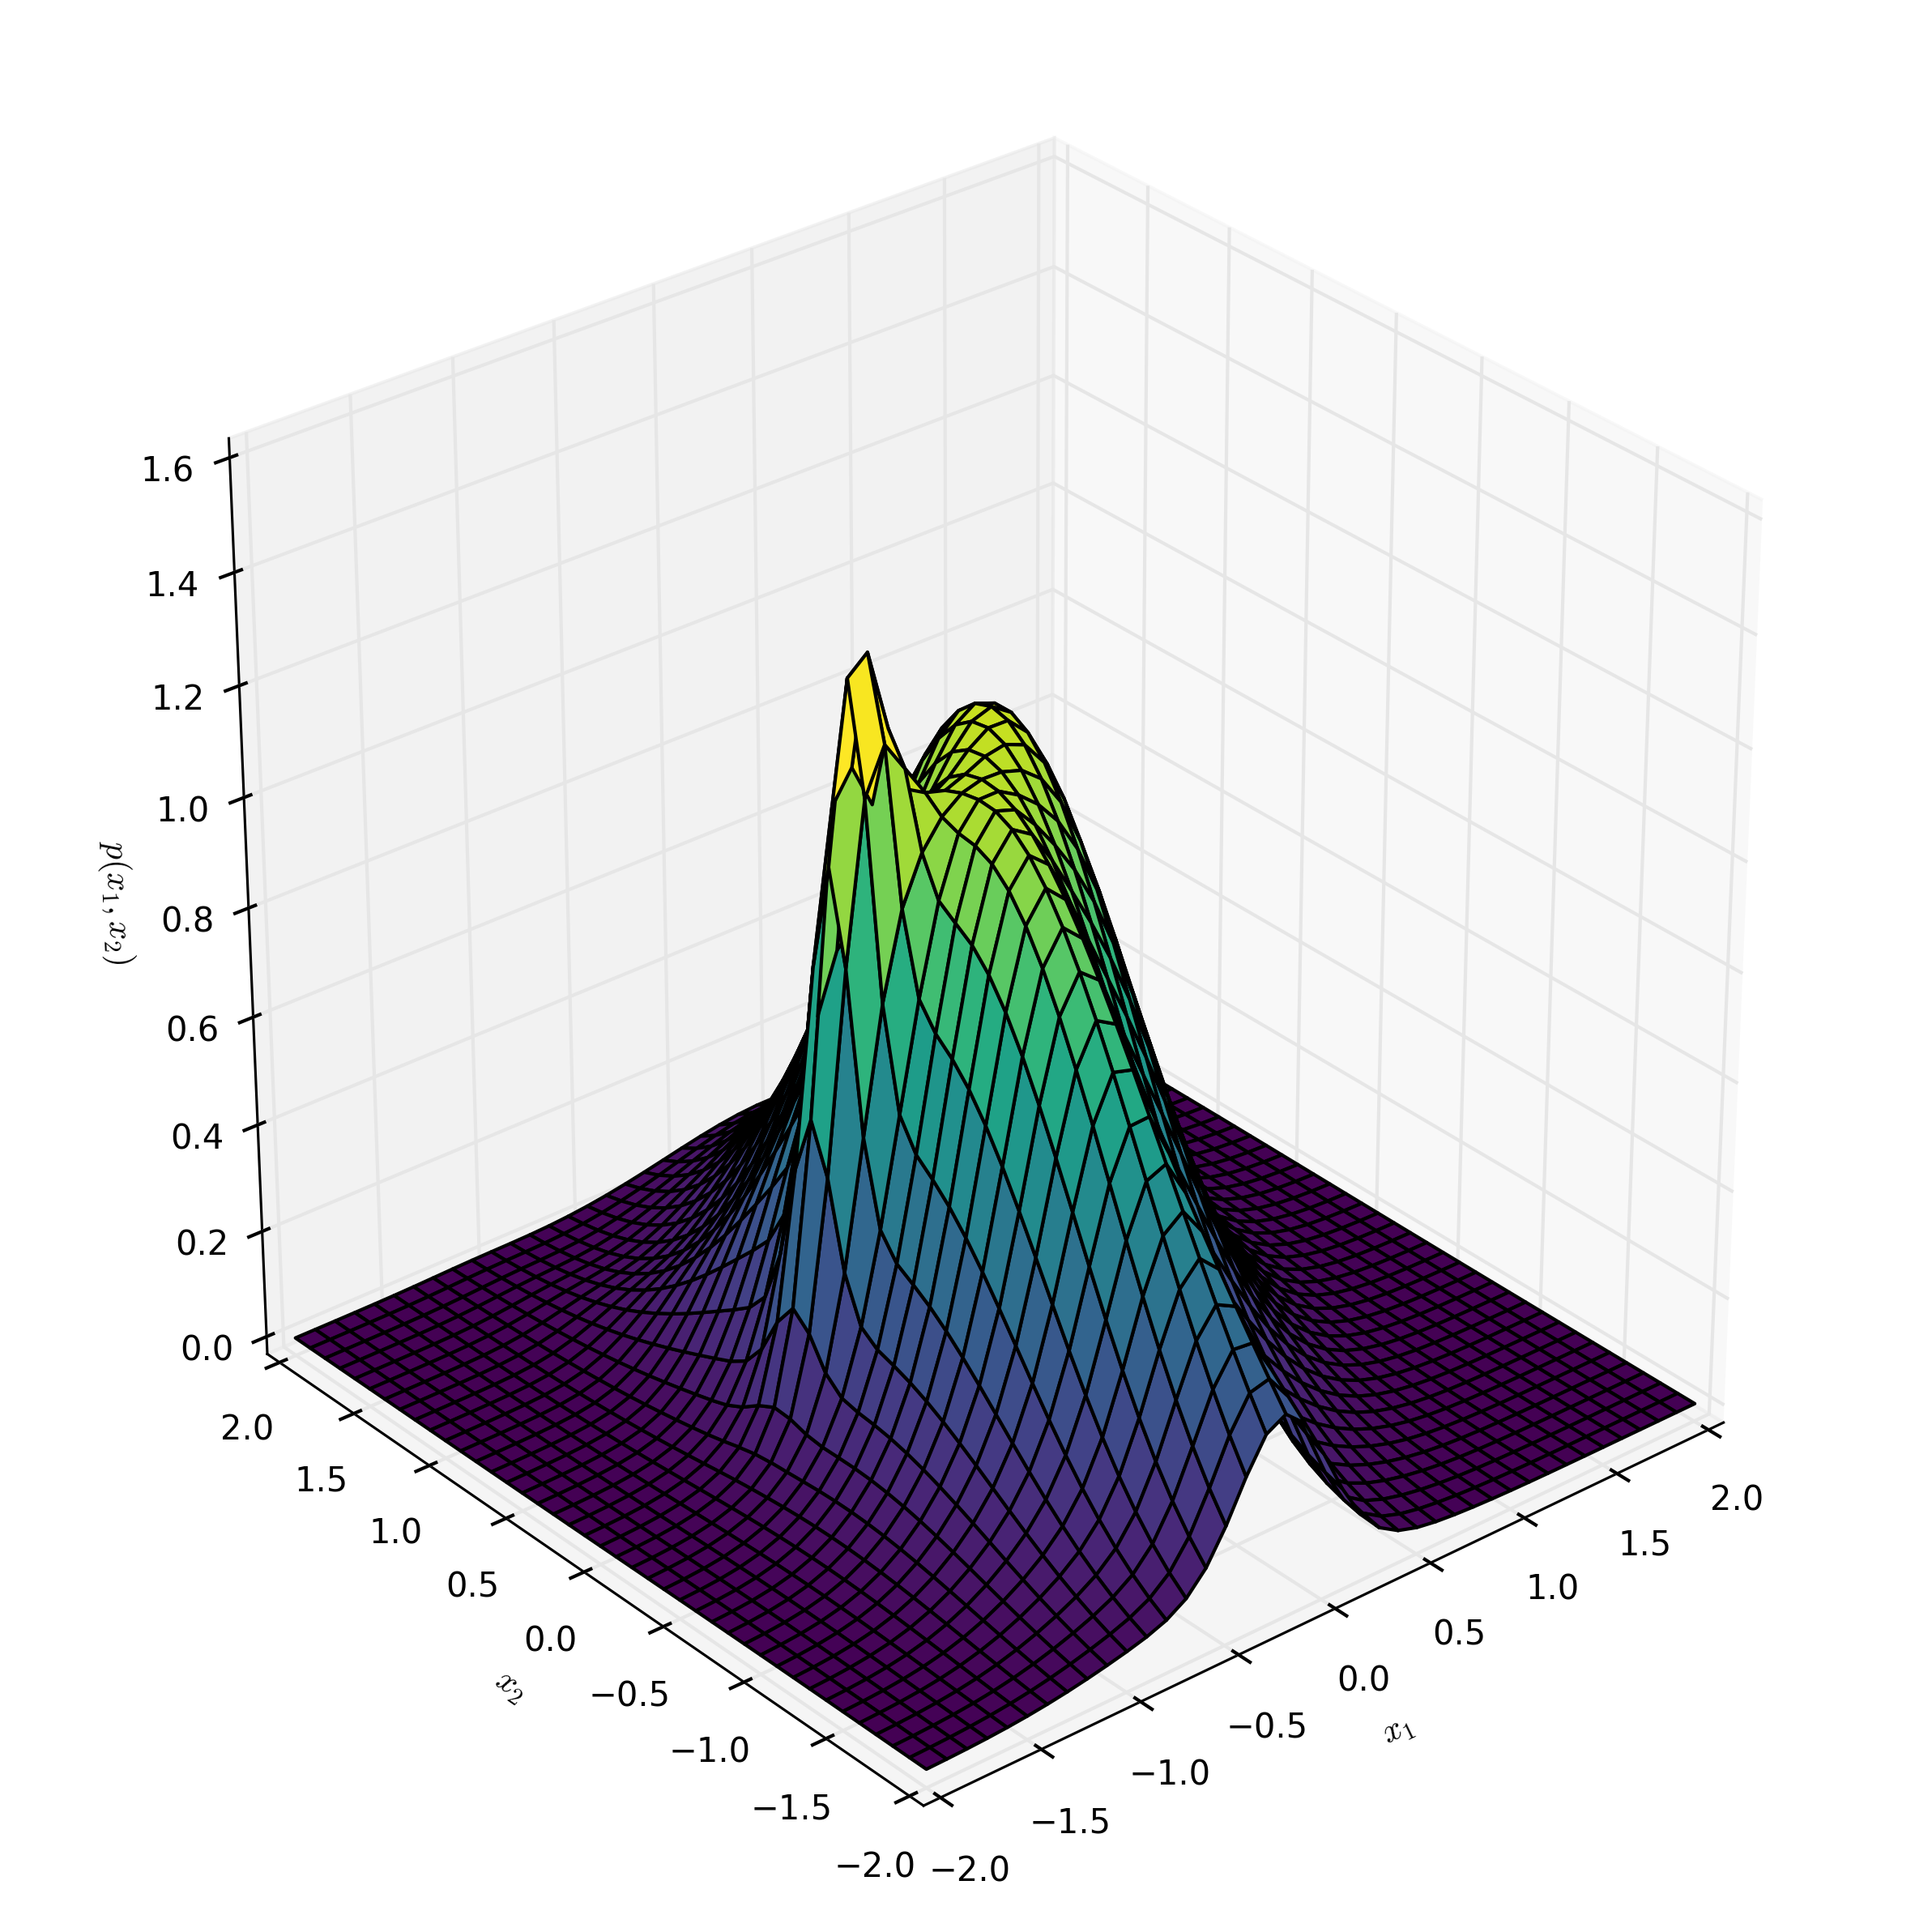
\includegraphics[width=.48\linewidth]{figures/mm.png}}
\subfloat[The output of the network after 2000 epochs with $M=40$ and $\eta=0.01$]{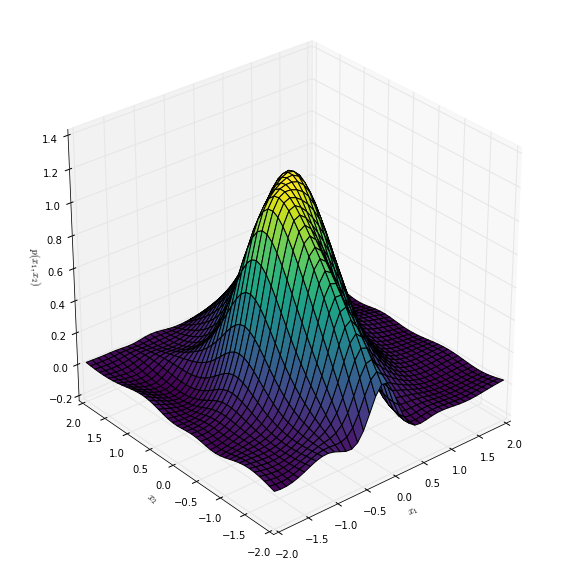
\includegraphics[width=.48\linewidth]{figures/mm_final.png}}
\caption{The original distribution and the distribution learned by an MLP.}
\label{fig:mm}
\end{figure}

\item The output from the network is quite similar to the original distribution. The major missing feature is the \emph{``peak''} in the original distribution. This peak is probably not smooth enough for the network to represent.

The network may converge faster if the root mean squared error is used instead of simply the sum of squares. The loss will be less noisy, because it is averaged over multiple training examples. To increase the performance, it may be beneficial to use a deeper, but more narrow network. I.e., increase the number of layers, but decrease the number of units per layer. This will increase the expressive power of the network, while requiring less hidden units than a 2 layer MLP. Lastly, the performance of the network can be increased by using more data. In this case, this can simply be achieved by increasing the number of samples taken from the original distribution.
\end{enumerate}


\pagebreak
\section*{Exercise 3 -- EM and doping} %%%%%%%%%%%%%%%%%%%%%%%%%%%%
\begin{enumerate}
\item 
Using the following code snippet we get the plot shown in Figure \ref{fig:expl}.
\begin{lstlisting}
X = np.loadtxt('a011_mixdata.txt')
df = pd.DataFrame(X, columns=[1, 2, 3, 4])
sns.pairplot(df)
\end{lstlisting}
 $x_1$, $x_2$ and $x_3$ seem to all be somewhat correlated. $x_4$ seems mostly uncorrelated with the other variables for the most part. It is hard to spot any meaningful structure with the naked eye. Figure \ref{fig:scatter} is more promissing. It is possible to make out some points that show signs of doping.
\begin{figure}
\centering
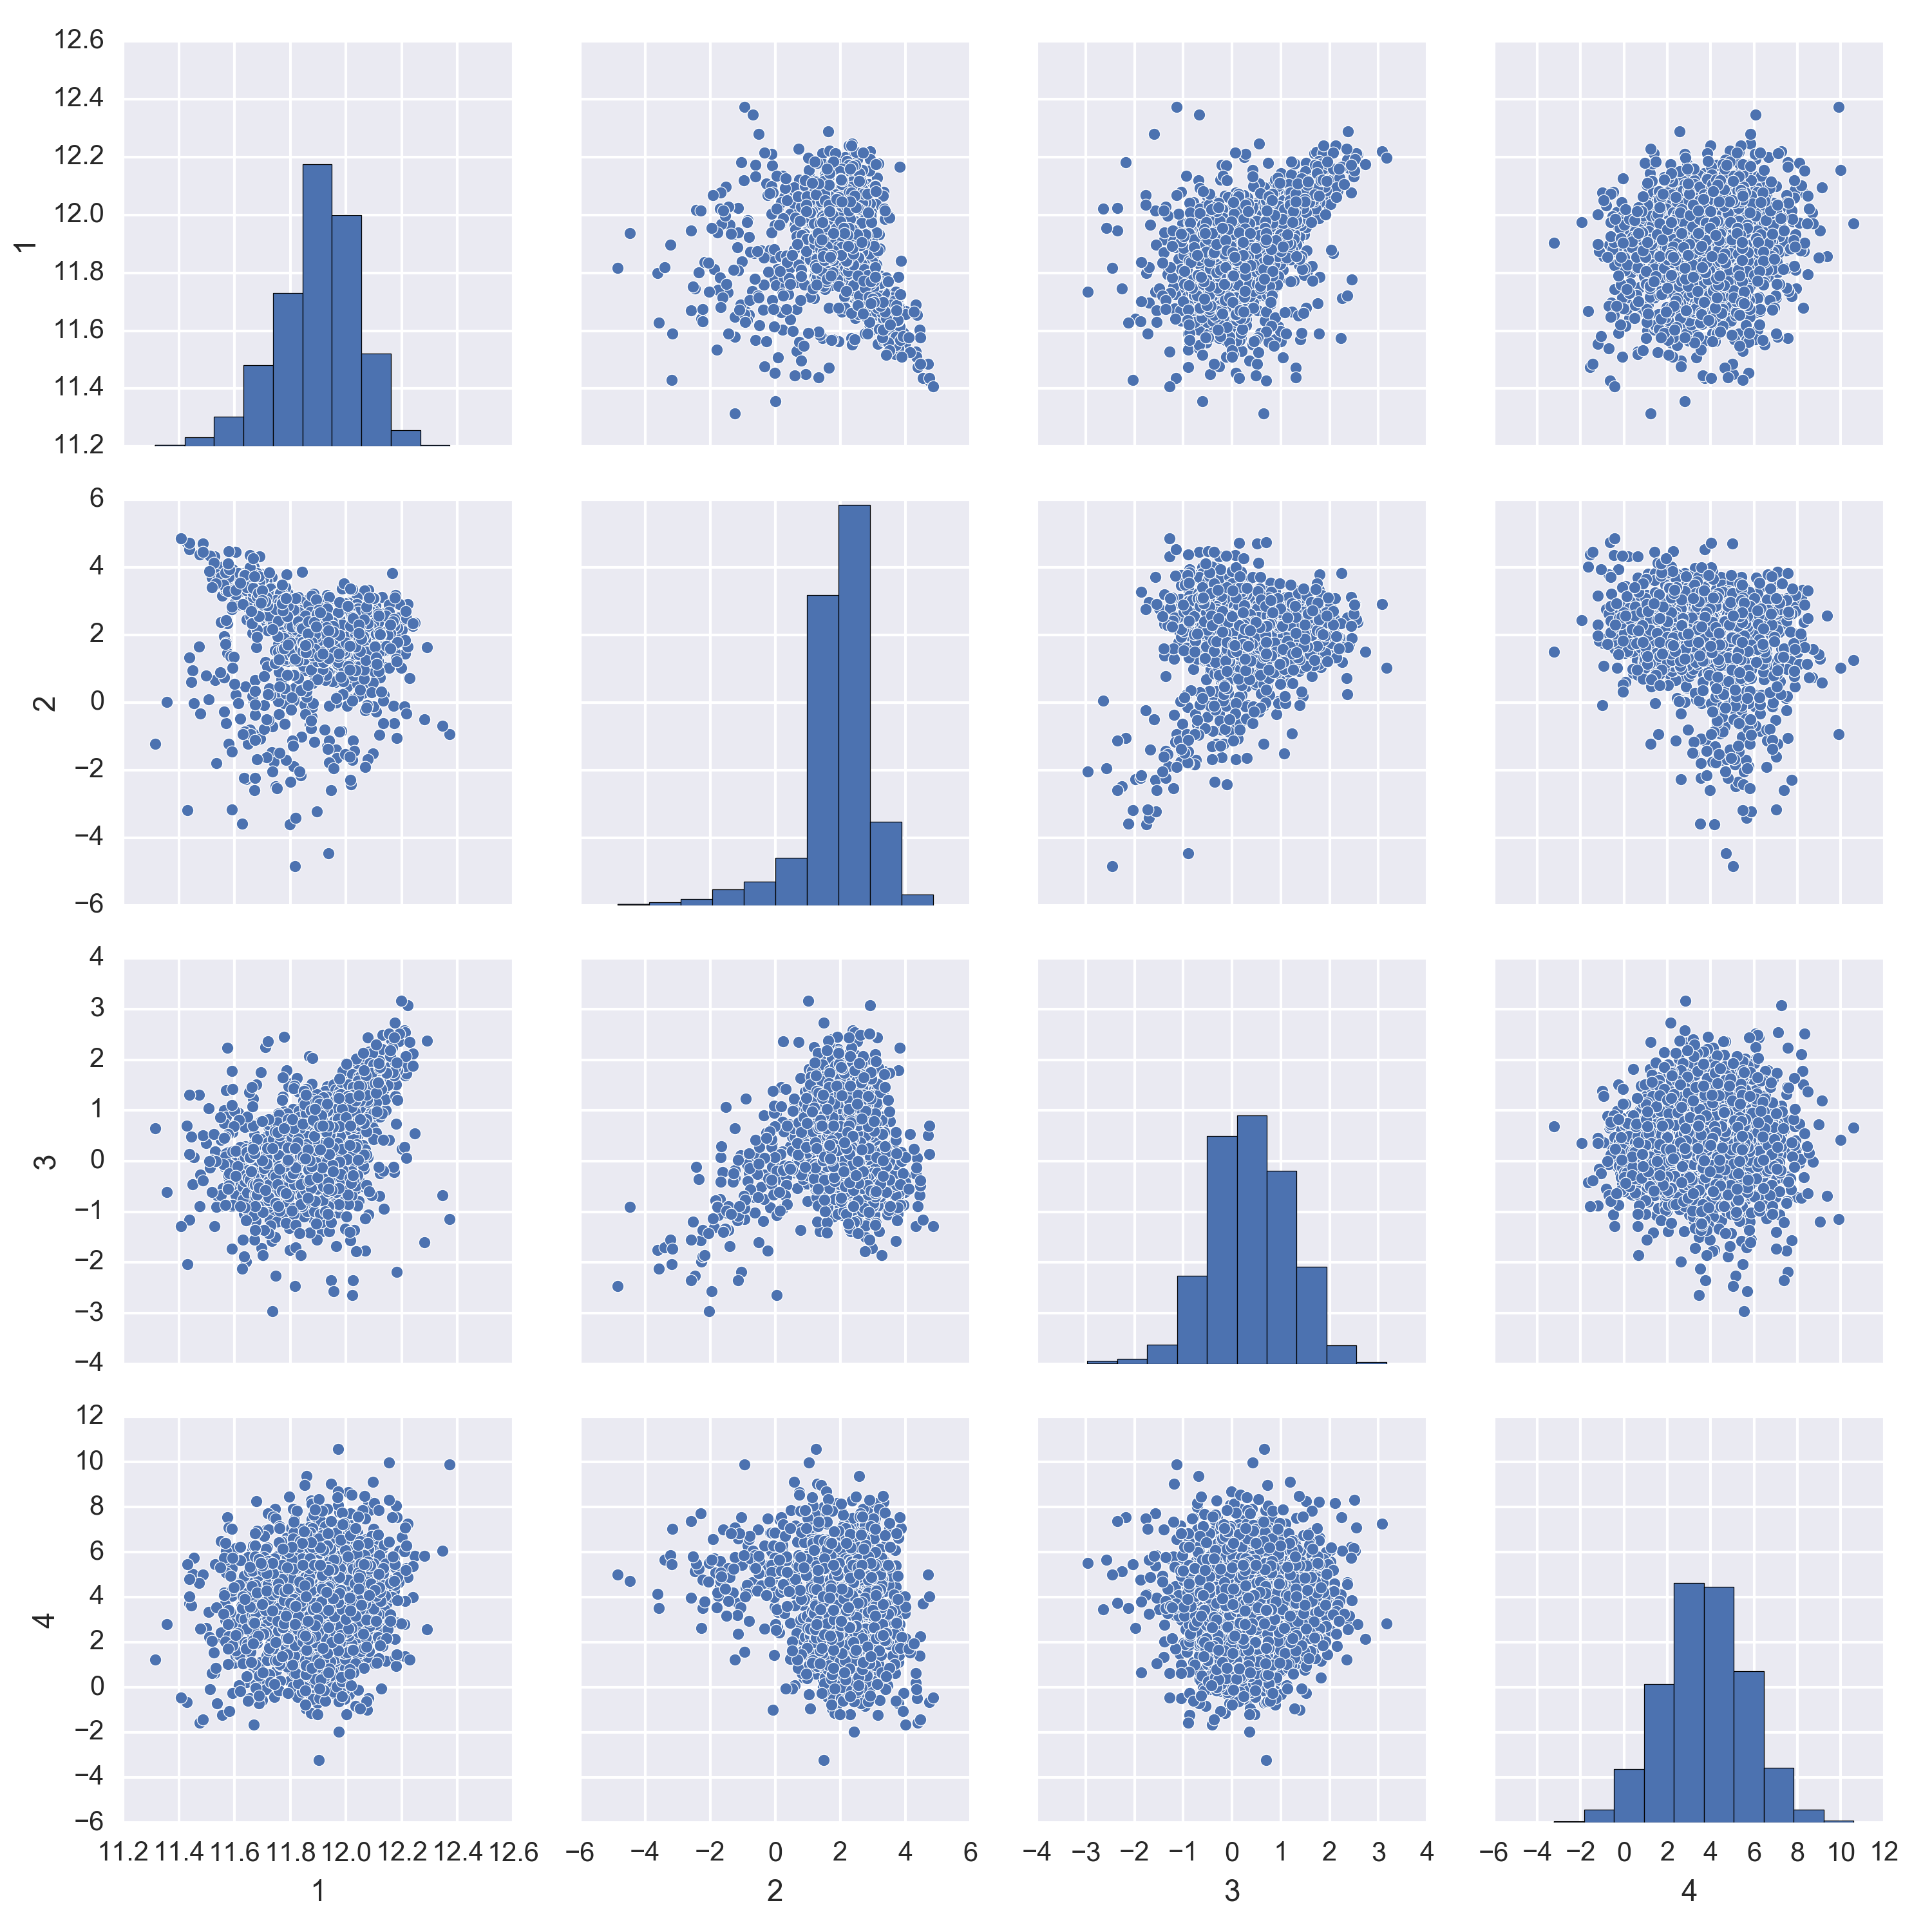
\includegraphics[width=\linewidth]{figures/EM_expl.png}
\caption{Scatter plots of all combinations of variables. On the diagonal a histogram of that single variable is shown.}
\label{fig:expl}
\end{figure}
\begin{figure}[H]
\centering
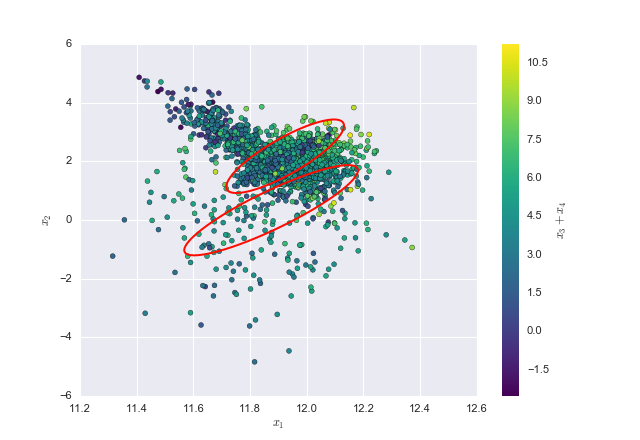
\includegraphics[width=.8\linewidth]{figures/scatter.png}
\caption{Scatter plot of $x_1$ and $x_2$. The points are coloured according to $x_3 + x_4$. The red ellipses indicate points which are positively correlated between $x_1$ and $x_2$, and also show some structure in $x_3 + x_4$. The bottom circle contains very few points ($\ll20\%$), so I think the top circle is more likely to be caused by subject X. These could be possible cases of doping. Other simple combinations of $x_3$ and $x_4$ did not show interactions like here.}
\label{fig:scatter}
\end{figure}
\item 
The code closely follows the summarization in Bishop \S9.2.2. The E step consists of evaluation the responsibilities
\begin{equation}
\gamma(z_{nk}) = \frac{\pi_k\mathcal{N}(\bm{x}_n|\bm{\mu}_k,\bm{\Sigma}_k)}{\sum_{j=1}^K\pi_j\mathcal{N}(\bm{x}_n|\bm{\mu}_j,\bm{\Sigma}_j)}.
\end{equation}
In the M step, the parameters are re-estimated
\begin{align}
N_k &= \sum_{n=1}^N\gamma(z_{nk}) \\
\bm{\mu}_k^{\text{new}}&=\frac{1}{N_k}\sum_{n=1}^N\gamma(z_{nk})\bm{x}_n\\
\bm{\Sigma}_k^{\text{new}} &= \frac{1}{N_k}\sum_{n=1}^N\gamma(z_{nk})(\bm{x}_n - \bm{\mu}_k^{\text{new}})(\bm{x}_n - \bm{\mu}_k^{\text{new}})^T \\
\pi_k^{\text{new}} &= \frac{N_k}{N}.
\end{align}
This translates to the following procedure
\begin{lstlisting}
# This function does proper broadcasting, which is
# very useful when computing the covariances
from numpy.core.umath_tests import matrix_multiply as mm

def EM(X, K=4, max_iter=100, tol=0.01):
    # Initialize variables
    N, D = X.shape
    pis = np.ones(K) / K
    mus = np.random.uniform(-1, 1, size=(K, D)) + X.mean(axis=0)
    covs = np.ones((K, D, D)) * (4*np.random.rand(D) + 2) * np.eye(D)
    
    prev_llh = 0
    for i in range(max_iter):
        # E step
        resps = np.zeros((K, N)) # responsibilities
        for k in range(K):
            resps[k] = pis[k] * multivariate_normal(mus[k], covs[k]).pdf(X)
        resps /= resps.sum(axis=0)
        
        # M step
        Nks = resps.sum(axis=1)[:, np.newaxis]
        mus = np.dot(resps, X) / Nks # Calculate new mus
        for k in range(K):
            diff = X - mus[k]
            sqdiff = mm(diff[:, :, np.newaxis], diff[:, np.newaxis, :])
            covs[k] = (resps[k, :, np.newaxis, np.newaxis] * sqdiff).sum(axis=0)
        covs /= Nks[:, np.newaxis]
        pis = Nks / N
        
        # Evaluate log likelihood
        llh = 0
        for pi, mu, cov in zip(pis, mus, covs):
            llh += pi*multivariate_normal(mu, cov).pdf(X)
        llh = np.log(llh).sum()
        print('Iteration: %d, likelihood %.4f' % (i, llh))
        
        if np.abs(llh - prev_llh) < tol:
            # Break if the log-likelihood hasn't improved much
            break
        prev_llh = llh
    
    return pis, mus, covs 
\end{lstlisting}
The following method creates a scatter plot of $x_1$ and $x_2$. Each point is colored by the index of the weighted gaussian that is most likely. 
\begin{lstlisting}
def plot_components(X, mus, covs, pis):
    N, K = X.shape[0], mus.shape[0]
    # Evaluate the model
    probs = np.zeros((K, N))
    for k in range(K):
        probs[k] = pis[k] * multivariate_normal(mus[k], covs[k]).pdf(X)
    prediction = np.argmax(probs, axis=0)
    
    plt.figure()
    colors = ['#E69F00', '#56B4E9', '#F0E442', '#009E73']
    for k, color in zip(range(K), colors):
        plt.scatter(X[prediction==k, 0], X[prediction==k, 1], c=color, label='C=%d'%k)

    plt.legend()
    plt.xlabel('$x_1$')
    plt.xlabel('$x_2$')
    plt.savefig('EM.png', dpi=300, bbox_layout='tight')
    plt.show()
\end{lstlisting}
\item Using $K=2$, the algorithm converges after 26 iterations. Running the algorithm with a different random seed resulted in swapping the means and covariances of the two gaussians with minor perturbations. The components shown in \ref{fig:K2} show correlations of $\rho_{12}=-0.33$ $\rho_{12}=-0.05$ respectively. No positive correlation is found.
\begin{figure}
\centering
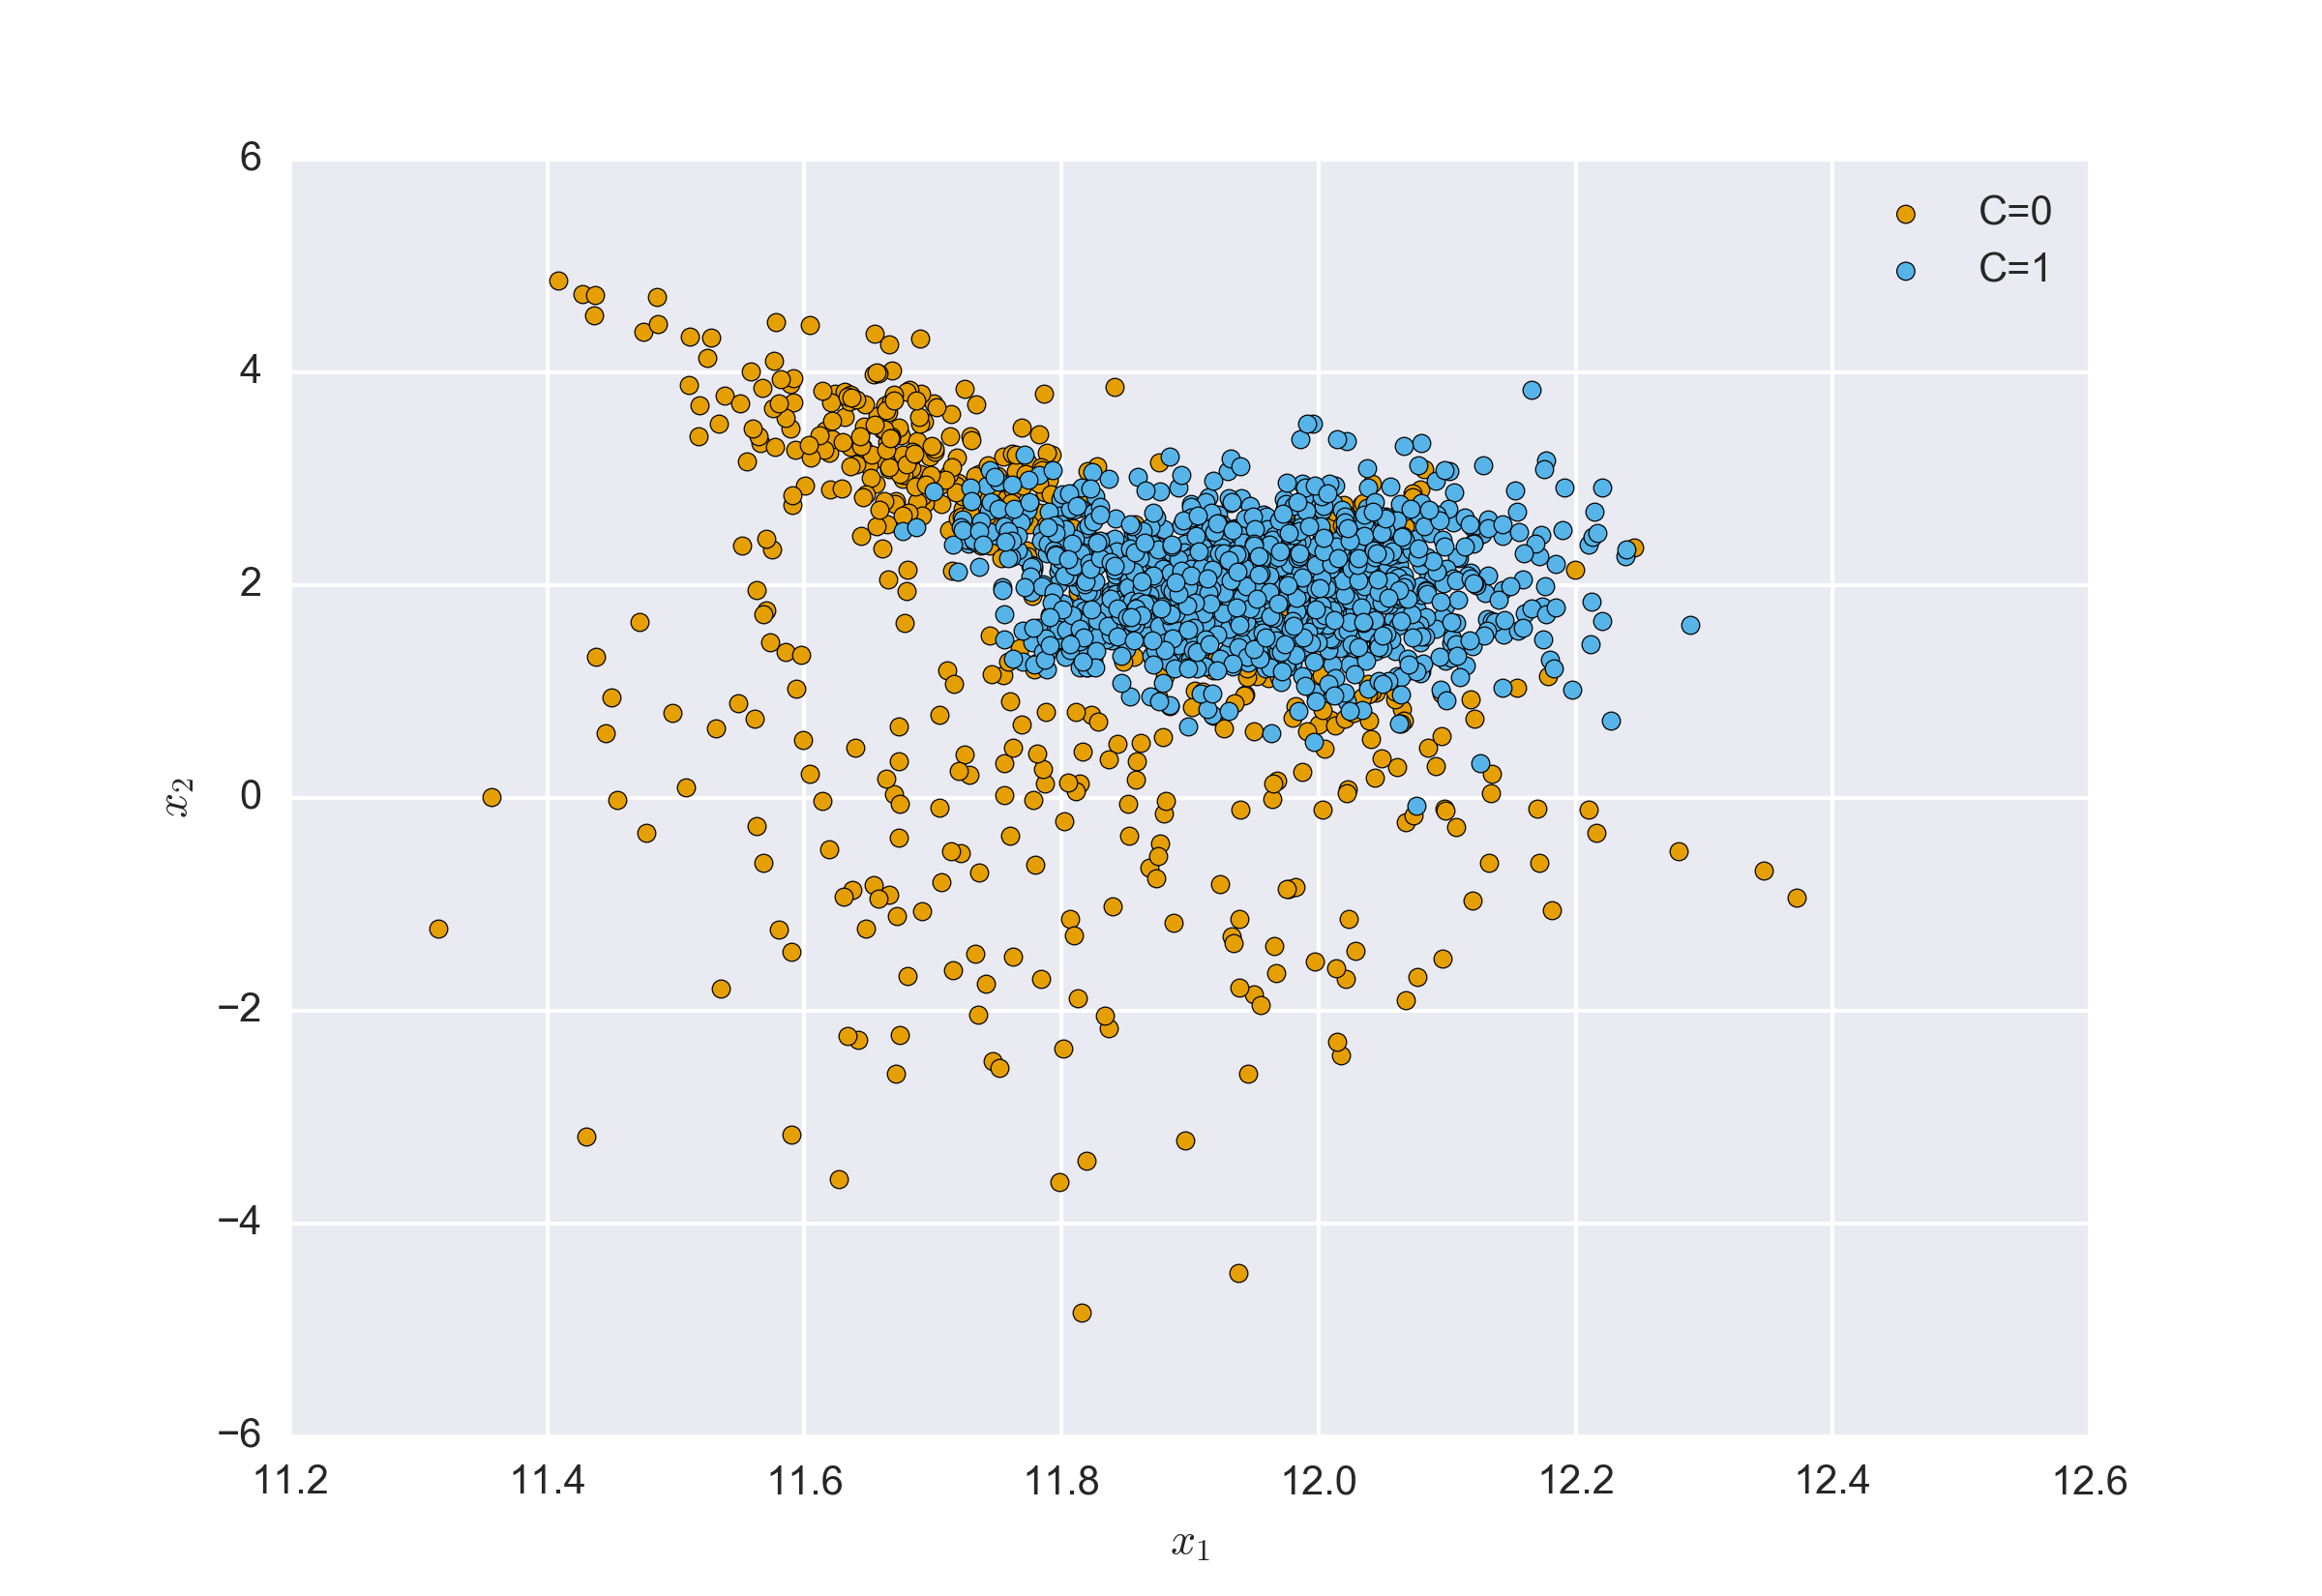
\includegraphics[width=0.8\linewidth]{figures/EM_K2.png}
\caption{Most probable components with $K=2$ after 26 iterations.}
\label{fig:K2}
\end{figure}
\item Increasing the number of components to $K=3$, we find the components shown in Figure \ref{fig:K3}. At this point, the highest correlation is just 0.08, i.e. we still haven't found the cluster we are looking for.
\begin{figure}
\centering
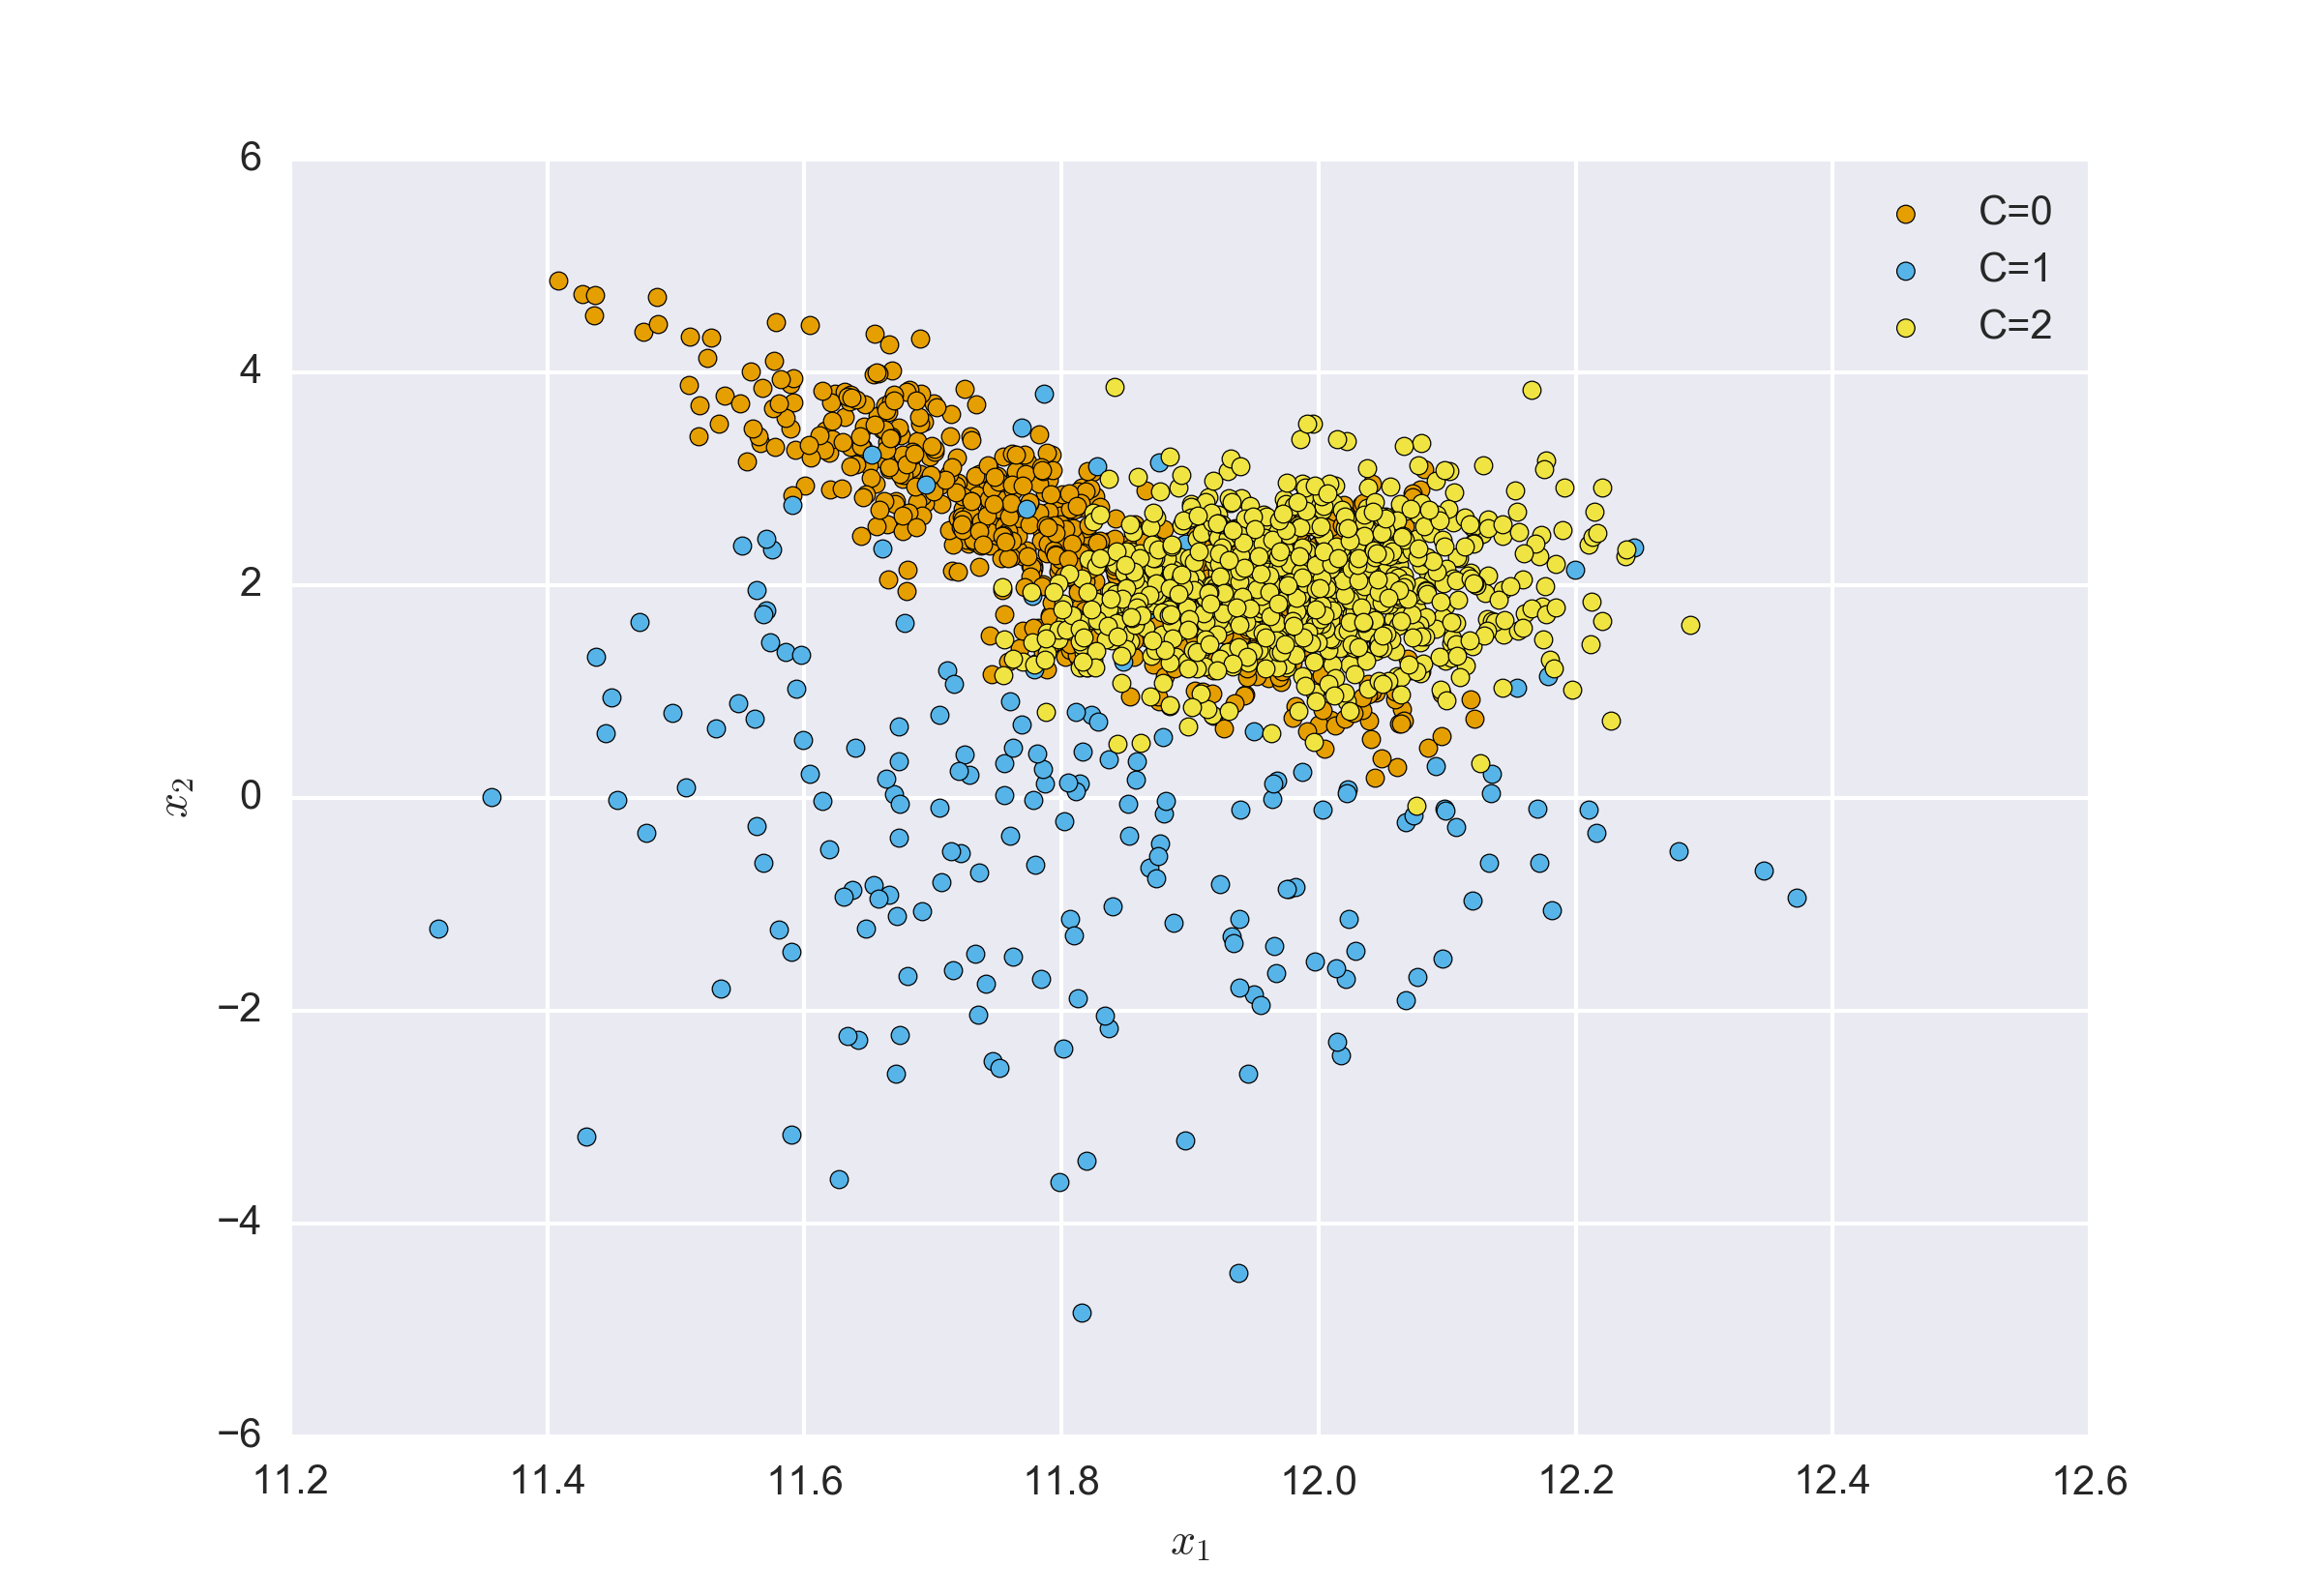
\includegraphics[width=0.8\linewidth]{figures/EM_K3.png}
\caption{Most probable components with $K=3$ after 22 iterations.}
\label{fig:K3}
\end{figure}
With $K=4$ components, the results are a lot more promising. Cluster 1 displayed in Figure \ref{fig:K4} has a correlation of 0.92. $21\%$ of the participants most likely belong to this cluster. This means that the rumour is very accurate (maybe even on the low side).
\begin{figure}
\centering
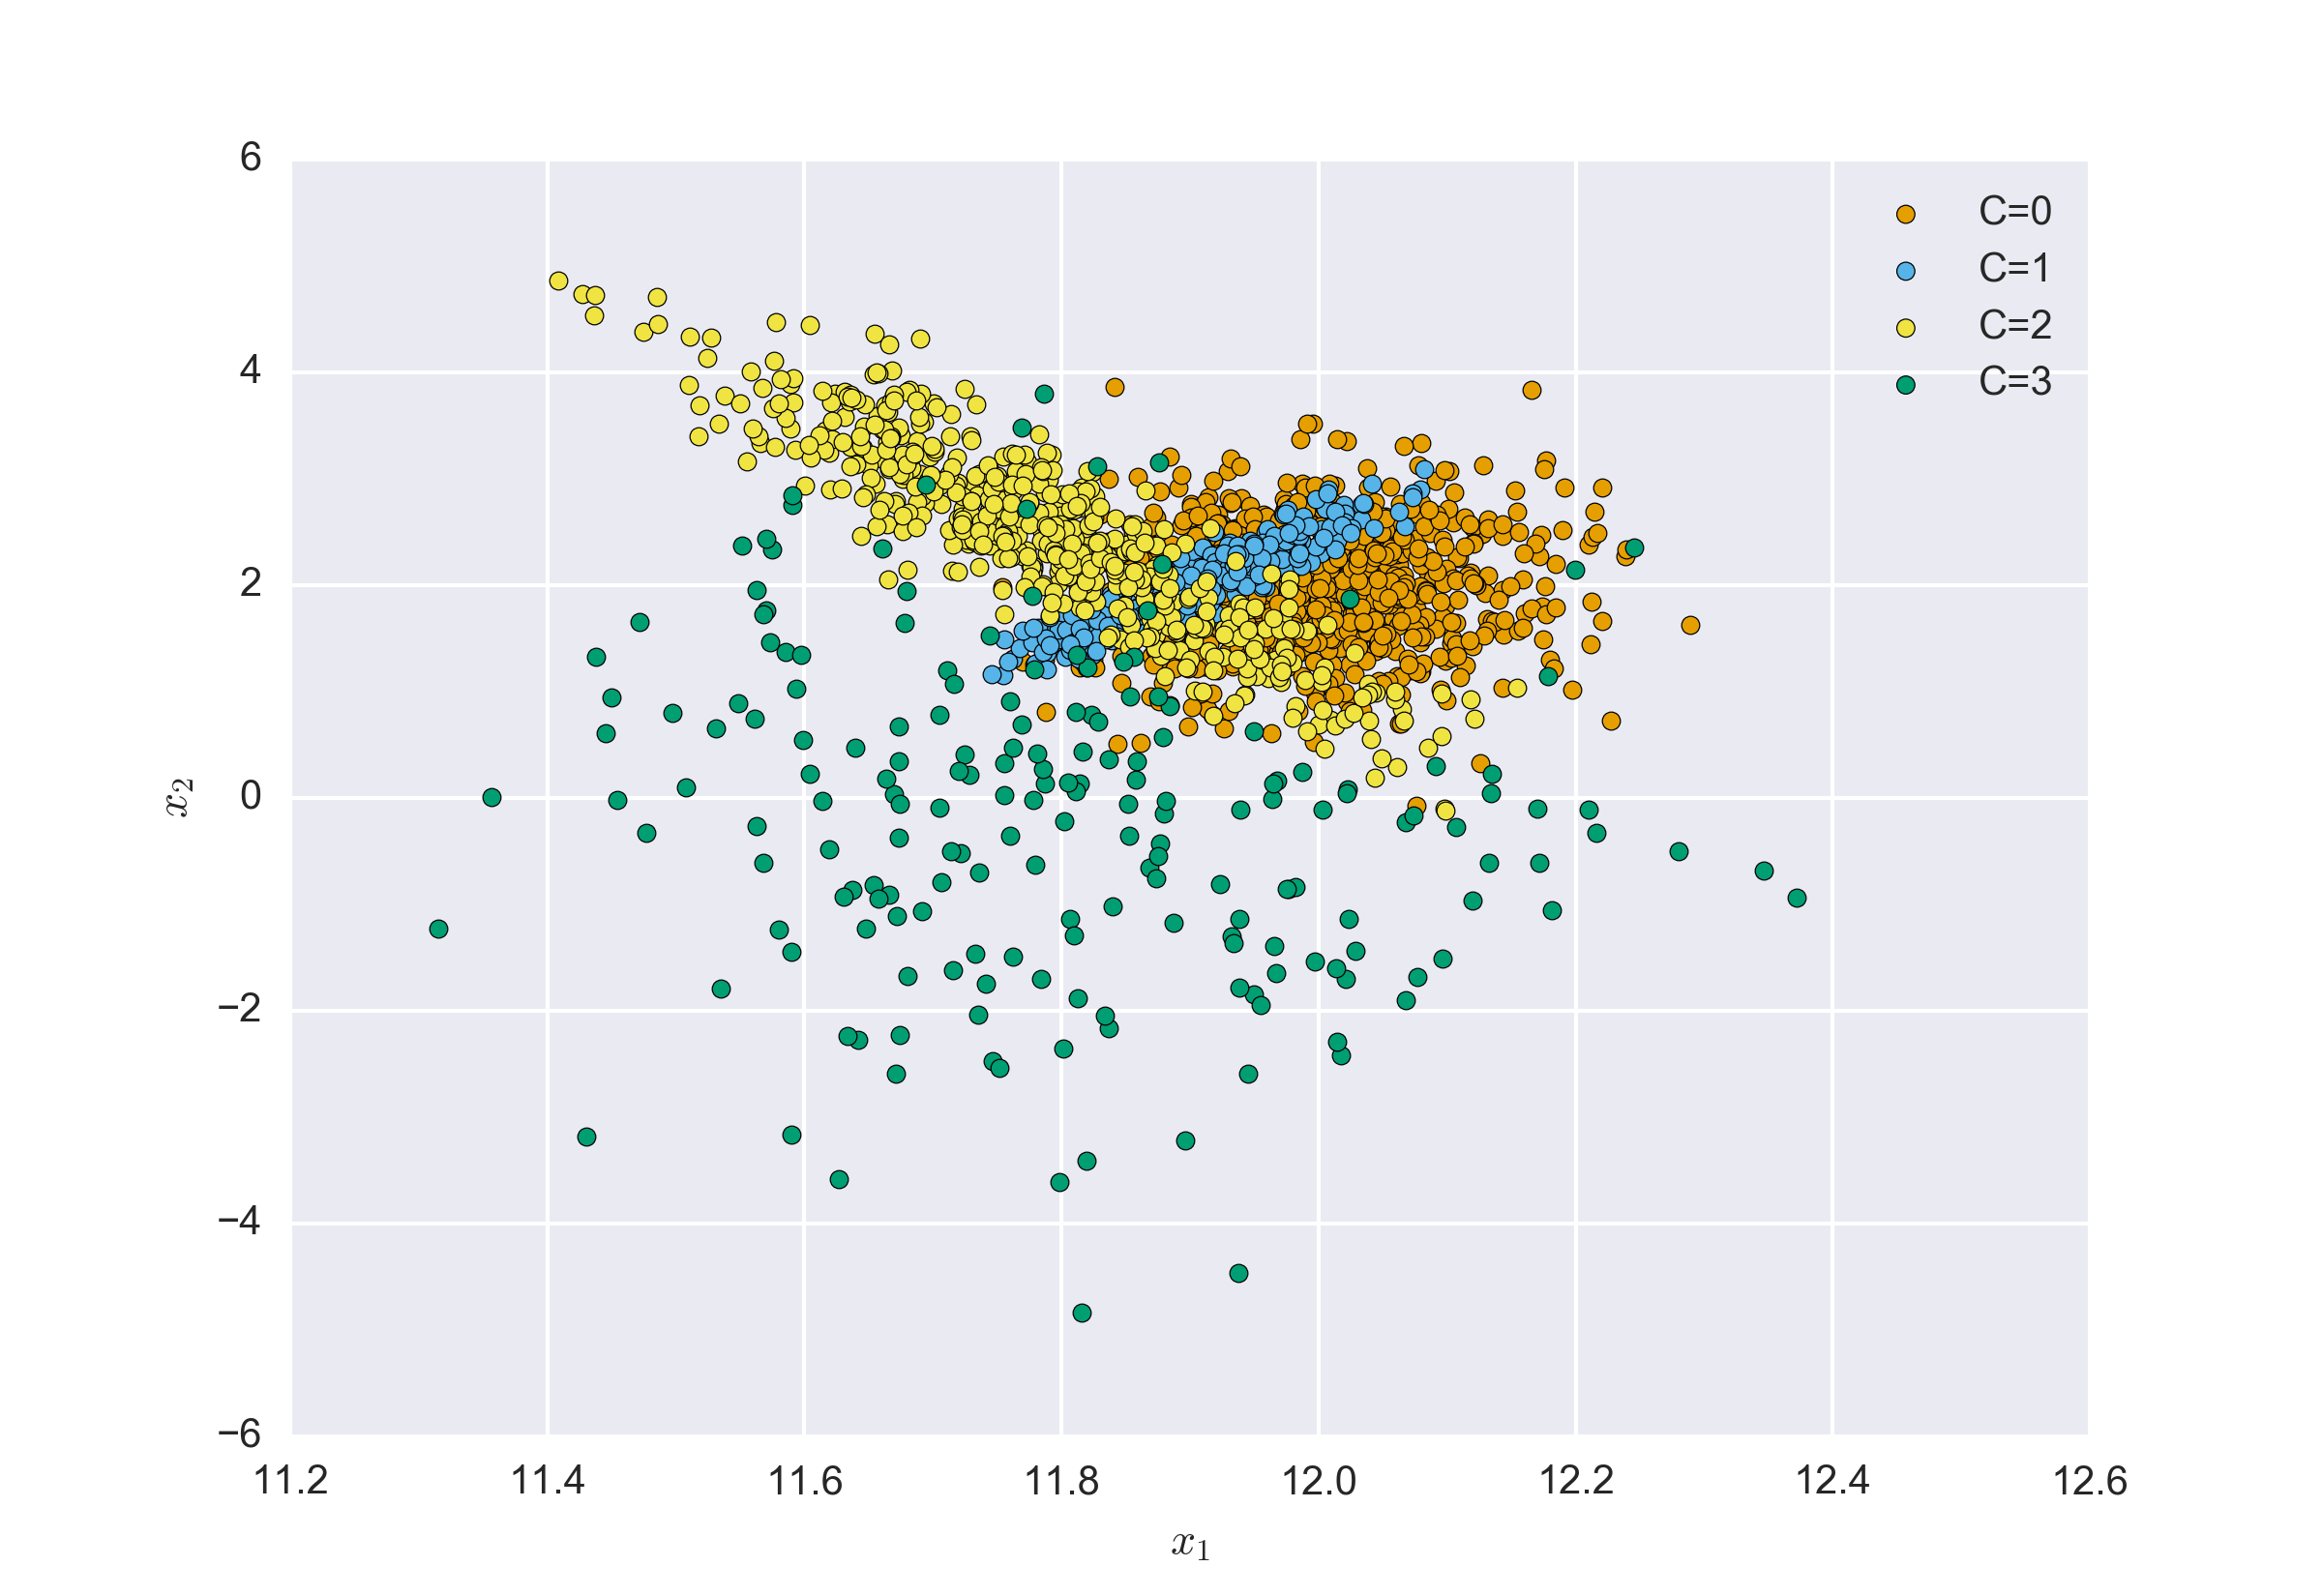
\includegraphics[width=0.8\linewidth]{figures/EM_K4.png}
\caption{Most probable components with $K=4$ after 55 iterations.}
\label{fig:K4}
\end{figure}
\item Sample C likely belongs to component 1, which means that they have taken drug X. Finding the fraud is a bit harder: both subjects B and D have a very low likelihood ($2.3\times10^{-35}$ and $1.5\times10^{-33}$ respectively). Subject B most likely belongs to component 2, which has a strong negative correlation. Subject D belongs to the 4th component, which is way more sparse. My guess would be that subject B is the fraud, based on the likelihood of the sample.
\end{enumerate}

\pagebreak
\section*{Exercise 4 -- Handwritten digit recognition} %%%%%%%%%%%%%%%%
\begin{enumerate}
\item The following code loads the digits and plots a few of them. The result can be found in Figure \ref{fig:digits}.
\begin{lstlisting}
N, D = 800, 28*28
with open('a012_images.dat', 'rb') as fid:
    X = np.fromfile(fid, np.uint8).reshape(N, D)

def plot_digit(X):
    plt.imshow(X.reshape(28, 28).T, cmap=plt.cm.Greys)
    plt.show()

for i in np.random.choice(N, size=5):
    plot_digit(X[i])
\end{lstlisting}
I think it should be fairly easy to classify the digits correctly. The digits in this dataset are very different from one another.
\begin{figure}
\centering
\subfloat{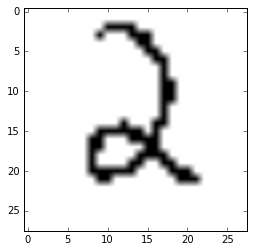
\includegraphics[width=.3\linewidth]{figures/dig2.png}}
\subfloat{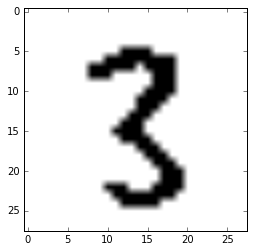
\includegraphics[width=.3\linewidth]{figures/dig3.png}}
\subfloat{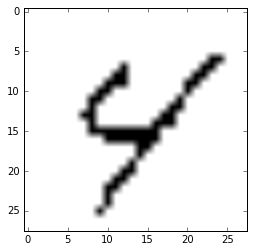
\includegraphics[width=.3\linewidth]{figures/dig4.png}}
\caption{An example of each digit in the dataset}
\label{fig:digits}
\end{figure}
\item The bernoulli distribution is given by
\begin{equation}
p(\bm{x}|\bm{\mu}) = \prod_{i=1}^D\mu_i^{x_i}(1 - \mu_i)^{(1 - x_i)}.
\end{equation}

In the E step, we once again evaluate the responsibilities
\begin{equation}
\gamma(z_{nk}) = \frac{\pi_kp(\bm{x}_n|\bm{\mu}_k)}{\sum_{j=1}^K\pi_jp(\bm{x}_n|\bm{\mu}_j)}.
\end{equation}

In the M step, we compute the new means and mixing coefficients
\begin{align}
N_k &= \sum_{n=1}^N\gamma(z_{nk}) \\
\bm{\mu}_k^{\text{new}} &=\frac{1}{N_k}\sum_{n=1}^N\gamma(z_{nk})\bm{x}_n \\
\pi_k^{\text{new}} &= \frac{N_k}{N}.
\end{align}

Using a bernoulli mixture model instead of a gaussian mixture model is only requires a few straightforward changes to the code. None of the techniques for countering extremely small likelihoods described in the assignment were necessary.

\begin{lstlisting}
from numpy.core.umath_tests import matrix_multiply as mm

def EM(X, K=4, max_iter=100, tol=0.01):
    # Initialize variables
    N, D = X.shape
    pis = np.ones(K) / K
    mus = np.random.uniform(0.25, 0.75, size=(K, D))
    
    prev_llh = 0
    for i in range(max_iter):
        # E step
        resps = np.zeros((K, N)) # responsibilities
        for k in range(K):
            resps[k] = pis[k] * np.prod(mus[k]**X * (1-mus[k])**(1-X), axis=1)
        resps /= resps.sum(axis=0)
        
        # M step
        Nks = resps.sum(axis=1)[:, np.newaxis]
        mus = np.dot(resps, X) / Nks # Calculate new mus
        pis = Nks / N
        
        # Evaluate log likelihood
        llh = 0
        for k in range(K):
            llh += pis[k] * np.prod(mus[k]**X * (1-mus[k])**(1-X), axis=1)
        llh = np.log(llh).sum()
        print('Iteration: %d, likelihood %.4f' % (i, llh))
        
        # Plot the means
        _, axs = plt.subplots(1, K)
        for mu, ax in zip(mus, axs):
            ax.imshow(mu.reshape(28, 28).T, cmap=plt.cm.Greys, vmin=0, vmax=1)
        plt.show()

        if np.abs(llh - prev_llh) < tol:
            # Break if the log-likelihood hasn't improved much
            break
        prev_llh = llh
    
    return pis, mus
\end{lstlisting}

\item Figure \ref{fig:means} shows the means after just 1 iteration and after 40 iterations. After 1 iteration, the left image already represents a 3. The other 2 images are a bit more vague. However, after 40 iterations they clearly resemble the other two digits in the dataset. The algorithm converges quite fast: after 10 iterations, hardly any improvement is made. Using a different random initializationm mainly effects the order and early shape of the components. After a few iterations, it doesn't make much of a difference.

\begin{figure}
\centering
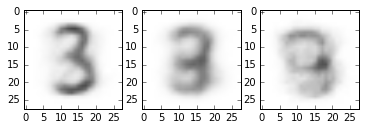
\includegraphics[width=.6\linewidth]{figures/means_init.png} \\
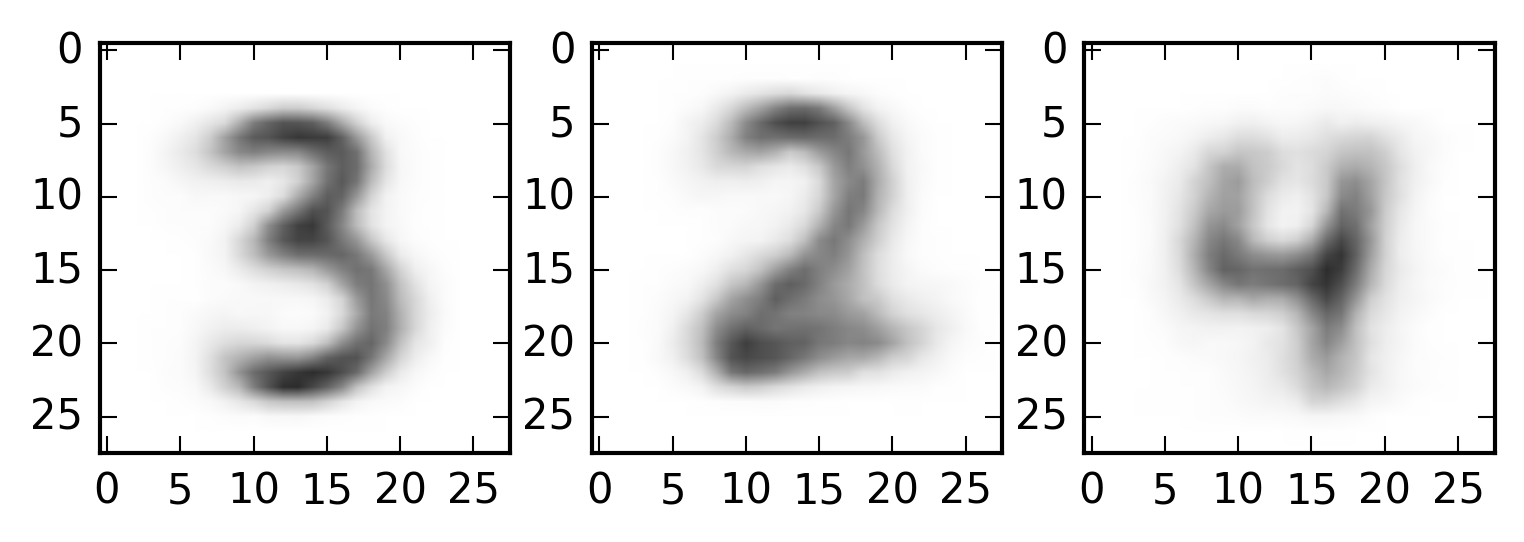
\includegraphics[width=.6\linewidth]{figures/means.png}
\caption{The means after 1 iteration (top) and after 40 iterations (bottom).}
\label{fig:means}
\end{figure}
\item Figure \ref{fig:diff_means} shows the results using 2 and 4 components. With 2 components, the 2 and 4 have merged into one component, while the 3 is still quite clear. This is probably because the 2 and 4 are more similar. When using 4 components, the results vary a lot between runs. In the case shown here, the component representing a 2 has very high probabilities. Other runs did not show behaviour like this. Usually, there were components for each digit and a ``rest'' component with digits that looked a bit dissimilar to the others.
\begin{figure}
\centering
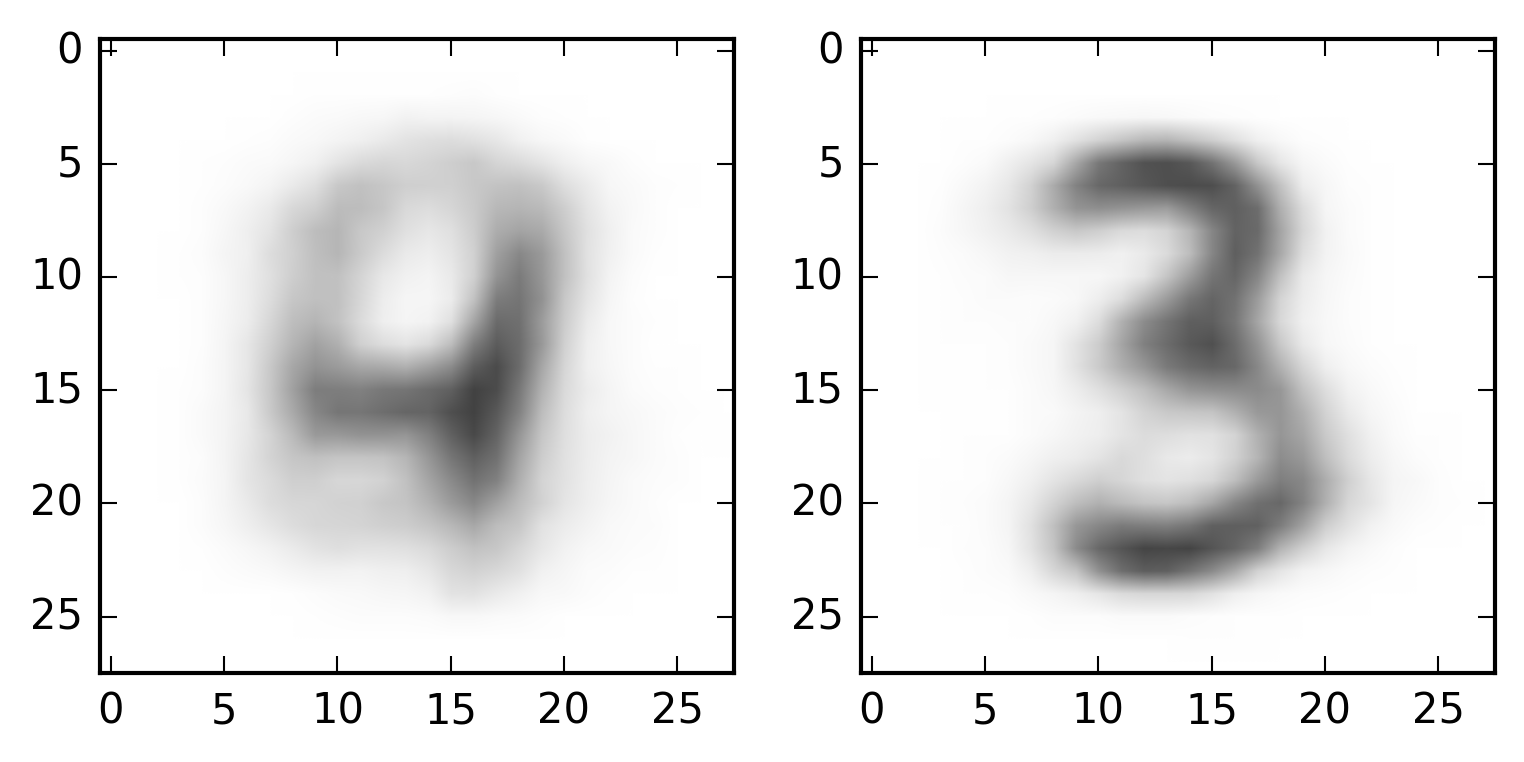
\includegraphics[width=.6\linewidth]{figures/means2.png} \\
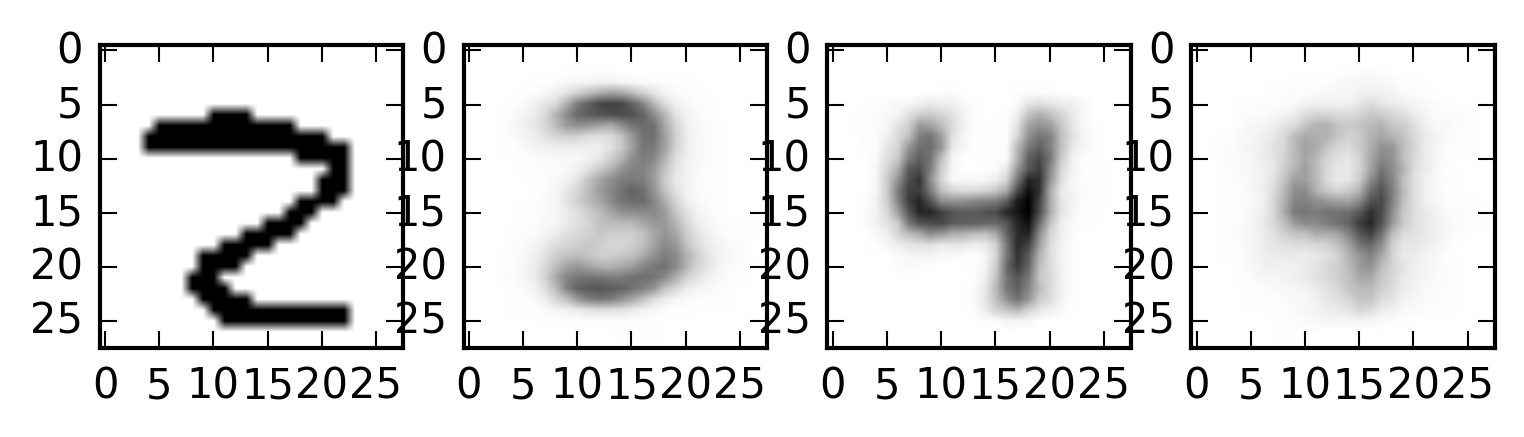
\includegraphics[width=.6\linewidth]{figures/means4.png}
\caption{The means using 2 components (top) and 4 components (bottom).}
\label{fig:diff_means}
\end{figure}

Using 3 components, the model made 125 errors in total (3 for digit 2, 103 for digit 3, and 19 for digit 4. See Figure \ref{fig:missers}). The 2s and 4s that were missclassified all looked very atypical compared to the rest of the dataset. For the 3s however, a lot of the mistakes looked like ordinary 3s. The reason for this is probably that the 3 has more within-class variance.

\begin{figure}
\centering
\subfloat[A 2 classified as a 4]{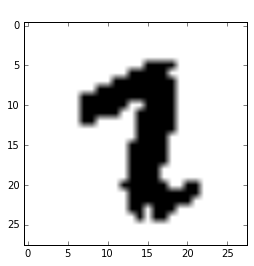
\includegraphics[width=.3\linewidth]{figures/miss2.png}}
\subfloat[A 3 classified as a 4]{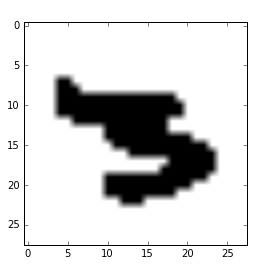
\includegraphics[width=.3\linewidth]{figures/miss3.png}}
\subfloat[A 4 classified as a 2]{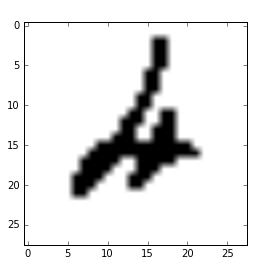
\includegraphics[width=.3\linewidth]{figures/miss4.png}}
\caption{A few digits that were missclassified by the model.}
\label{fig:missers}
\end{figure}

Lastly, we can initialize the means to the true values by taking the average image in each class. Now, the algorithm converges after only 4 iterations. The reason that 4 steps are still necessary is probably because of numerical issues.
\begin{lstlisting}
# Initialize with the true means
mus = np.vstack((np.mean(X[Z==2], axis=0),
                     np.mean(X[Z==3], axis=0),
                     np.mean(X[Z==4], axis=0)))
\end{lstlisting}

\item I have drawn a 2 (Figure \ref{fig:mydigit}). The model correctly classifies this to be in the component initialized with the mean of all other 2s.

\begin{figure}
\centering
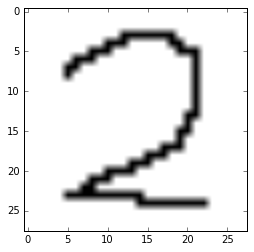
\includegraphics[width=.3\linewidth]{figures/mydigit.png}
\caption{A beautiful 2 drawn by myself}
\label{fig:mydigit}
\end{figure}
\end{enumerate}
\end{document}